\documentclass[man,floatsintext,donotrepeattitle]{apa6}

\usepackage{xfrac}
\usepackage{textcomp}
\usepackage[american]{babel}
\usepackage[utf8]{inputenc}

% Single space after period (Mike prefers)
\frenchspacing

% http://tex.stackexchange.com/questions/36423/random-unwanted-space-between-paragraphs
\raggedbottom

% ref: http://tex.stackexchange.com/questions/28516/how-to-change-the-title-of-toc
\addto\captionsamerican{% Replace ``english'' with the language you use
  \renewcommand{\contentsname}%
  {Table of Contents}%
}

%\usepackage[compact]{titlesec}
\usepackage{tabu}
\usepackage{amssymb,amsmath}
\usepackage{setspace}

% ref: http://tex.stackexchange.com/questions/48509/insert-list-of-figures-in-the-table-of-contents
\usepackage[nottoc,numbib]{tocbibind}

\usepackage[hyphens]{url}

% ref: http://tex.stackexchange.com/questions/73862/how-can-i-make-a-clickable-table-of-contents
\usepackage{hyperref}
\hypersetup{
  colorlinks,
  citecolor=black,
  filecolor=black,
  linkcolor=black,
  urlcolor=black
}
%\hypersetup{linktocpage}

%\usepackage{breakurl}
\usepackage{subfigure}
\usepackage{graphicx}
\usepackage[group-separator={,}]{siunitx}
\RequirePackage[l2tabu, orthodox]{nag}
\graphicspath{{./figures/dissertation/}} % Specifies the directory where pictures are stored

\usepackage{csquotes}
\usepackage[style=apa,sortcites=true,sorting=nyt,backend=biber,doi=false,uniquename=false]{biblatex}
\DeclareLanguageMapping{american}{american-apa}

\addbibresource{bibliography.bib}

% Needed to ensure periods are placed at the end of every bibliography entry in the references section
\AtEveryBibitem{\clearfield{doi}}

% Make sure only urls that are printed in references section are for webpages
\AtEveryBibitem{
  \ifentrytype{misc}{}{
    \clearfield{url}
  }
}

% ref: http://tex.stackexchange.com/questions/128592/remove-backslashes-from-url-fields-in-bib-entry
\DeclareSourcemap{
  \maps[datatype=bibtex]{
    \map{
      \step[fieldsource=url,
	match=\regexp{\\},
      replace=\regexp{}]
    }
  }
}

% Don't let biblatex change any of the casing in the bibliography file
\DeclareRobustCommand{\MakeSentenceCase*}[1]{{#1}}

% If the toc is too detailed, try limiting the depth of printed sections in the TOC:
\setcounter{tocdepth}{2}

\title{Comparing vector-based and ACT-R memory models of tag retrieval:\protect\\User-customized hashtag/tag prediction on Twitter and StackOverflow}
\shorttitle{Comparing memory models of tag retrieval}
%\shorttitle{}

\author{Clayton Stanley}
\affiliation{Rice University}

\leftheader{Beitzel}


%\keywords{}

\begin{document}

\abstract{
  This research aims to develop and compare tag-recommendation models for users choosing hashtags when composing a tweet on Twitter and choosing tags when asking a question on the StackOverflow site.
  Two state-of-the-art cognitively-plausible memory models will be evaluated on how accurate they predict a user's chosen tags: an ACT-R inspired Bayesian model and a random-permutation vector-based model.
  Experiments are designed to [1] discover the best way to leverage a user's prior hashtag use as a future predictor, [2] improve the models so that each model's strengths are incorporated into the other,
  and [3] formally evaluate and compare each model's performance when recommending hashtags on Twitter and tags on StackOverflow.
  The user-customized tag-recommendation models developed with this research should be immediately useful as foundations for tag-recommendation systems on the popular Twitter and StackOverflow social media sites.
  Further, the planned performance modifications to the two memory models are aimed at the architectural level of each model.
  If these architectural modifications to two cognitively-plausible memory models significantly improve performance,
  they may suggest task-independent general modifications that can help improve model fit to human data in a much wider range of domains.
}

\note{\today}

\maketitle

\tableofcontents
\newpage

\listoftables
\newpage

\listoffigures
\newpage

\section{Motivation}

The ACT-R cognitive architecture \parencite{Anderson2007} contains one of the leading theories of human declarative memory.
The declarative memory component in ACT-R is a Bayesian statistical model.
This is the same type of co-occurrence Naive Bayes statistical model that is prominent in the more general machine-learning field.
When these Bayesian models are used for machine learning, it is common to use a large number of observations to construct the co-occurrence matrix that is the foundation for the model.
The primary reason for this is that the stability of statistical models increase as sample size increases.

However, it is much less common in the cognitive modeling community to use a large number of observations to build up declarative memory when creating ACT-R models.
If a cognitive modeler is using the declarative memory component of ACT-R,
it is common to either construct the co-occurrences by hand, or use a small training set of data to initially build up the declarative memory system.
This approach can and has worked well.
Essentially the modeler is only including the observations in declarative memory that are relevant to the specific task that they are studying.

This approach is problematic for two main reasons:
First, it means that the declarative memory system for every developed model must be hand crafted and customized for that model, which takes enormous time and effort.
Second, it means that modelers are continuing to use small sample sizes for the declarative memory components in their models.

This has important implications for understanding declarative memory:
First, it is difficult to verify and explore modifications to the declarative memory architecture because the dataset is not large enough or rich enough to rigorously test modifications to the theory.
It also means that we do yet fully understand how well the ACT-R declarative memory theory scales when the number of chunks begins to approach the number of chunks that are actually stored in human declarative memory.

There is, however, an opportunity to change this approach.
With the massive growth of human-created content on social media sites (e.g., Twitter, StackOverflow, Wikipedia), and public access to many of those databases,
it is now possible to evaluate psychological theories of declarative memory on large-scale real-world tasks where the theory can be tested on hundreds of millions to billions of data points.
This will provide a way to test if these models scale, and evaluate the psychological validity of these models as the number of observations used increases by orders of magnitude.

A few researchers have started to use these large databases to evaluate how well declarative memory models scale,
for both ACT-R Bayesian models \parencites{Fu2007,Pirolli2003,Stanley2013,Douglass2010} and vector-based memory models \parencites{Jones2007,Rutledge2008,Recchia2010,Sahlgren2008}.

The work for this proposal will expand on previous work that has tested retrieval models on large-scale datasets.
It will focus specifically on how two state-of-the-art declarative memory retrieval models (ACT-R Bayesian and random permutations) can be improved, by testing these models on two real-world tagging tasks.
One primary objective is to compare the random-permutation vector-based model to ACT-R's declarative memory theory when large datasets are used for each model. 
Another objective is to improve each model, and measure how incorporating the strengths of each model into the other (i.e., modifying model components) influences accuracy.
For example, it is currently unexplored how a vector-based model can be modified to retrieve results that are based not only on context, but also on the prior odds that a particular item in memory will be needed again.
Large-scale datasets will be used throughout the model development and evaluation process.
This provides an ideal testing environment for constraints and assumptions for each theory to be rapidly tested and new model components to be hypothesized and quickly evaluated.

\subsection{Motivation for Task}

Social media sites such as Twitter, Facebook, StackOverflow, Google+, and Yelp are composed almost entirely of human-created content.
The amount of user content on these sites is staggering, and continues to grow.
Users of Twitter's microblogging service, for example, generate half a billion tweets per day \parencite{TwitterReport2012}.
However, a single user of a social media site is most likely interested in only a small fragment of this large amount of information.
One general question to support the user in this domain is:
How can we quickly and effectively connect users to the content that they care about?

A growing number of users on social media sites are focusing on and looking for recently created information when performing a search \parencite{Jansen2011}.
In other words, users on social media sites want the fresh \emph{stream} of information about a particular topic.
This can certainly be seen in the main user-interface views that these social media sites provide:
Twitter's homepage showing followees' tweets, Facebook's homepage showing friends' posts, and StackOverflow's daily digest of posts for particular tags.

So how can we ensure that users are connected to the information streams that they care most about?
One promising approach is to model and predict the user's goals when using and searching these social media sites \parencite{Rose2004}.
If we have a better understanding of a user's goals, then we can tailor the information streams provided to the ones that are most in line with these goals.
For example, Twitter might suggest other users and hashtags for the user to follow, Facebook could suggest pages to like, Yelp could recommend businesses to check out.
Researchers are currently looking for ways to automate the goal-identification task for more general search queries like those generated for Google \parencites{Jansen2008}{Lee2005}.

However, social media sites have an advantage over traditional search engines for identifying user goals: human-created content.
Twitter has more than just the tweet that a user is currently composing to try and identify that user's goals.
The site also has all of the user's previous content, and can use that information to provide a much better prediction of a user's goals.
Further, sites like Twitter, StackOverflow, Google+, and Facebook support ways for the user to explicitly identify their precise goals when creating content: hashtags.
These user-created hashtags are a key indicator of a user's goals on a social media site. 

These hashtags relate to a user's goals and interests because they are a form of human-based document tagging \parencite{Chang2010}.
Further, people are using hashtags as a way to create information streams on social media sites \parencite{Kwak2010}.
Twitter users, for example, commonly create and use hashtags for upcoming political events that interest them, such as debates and races \parencite{Diakopoulos2010}.
So if we can predict what hashtags a user is interested in, we have a better understanding of the information streams that they care about.
With that understanding, we can tailor the system to suggest hashtags that they may not yet know about but are of likely interest to them.
We can help aid in their discovery of fresh and relevant information that matches their goals on the site.

\subsection{Research Questions}

The core research question motivating this proposal is:
What kinds of cognitively-plausible models can best predict the human-created tags that a user on a social media site uses?
This question can be tested by generating a prediction for the most likely used hashtag whenever a user is about to generate a hashtag, and then comparing the user's chosen hashtag to the model's prediction.
This process can be framed as a memory retrieval problem.
That is, each user on a social media site has created content that contain a set of human-created tags within the context of each post.
The process of suggesting a relevant hashtag to a user can be thought of as a memory retrieval request for a hashtag, given prior hashtag use and current context.

Co-occurrence-based modeling has been shown as a potentially useful approach when predicting Twitter hashtag use \parencite{Efron2010}.
Several memory retrieval models are based on this broad methodology, where a count is maintained of the times each contextual element (such as a word in a post) co-occur with a tag.
Two of the current state-of-the-art memory retrieval models are based on a co-occurrence methodology, and I will be comparing these two models for hashtag prediction:
ACT-R's declarative memory (DM) retrieval theory and random permutation vector-based memory systems.

\subsubsection{StackOverflow and Twitter}

I will compare these two memory systems across two domains where users generate tags for posts: Twitter and StackOverflow.
Twitter is a microblogging service where users create 140 character tweets and broadcast those messages out to the users who follow their posts.
A user is free to annotate important concepts or words in the tweet by preceding words with hashtags ``\#''.
After the tweet is created the hashtags become hyperlinks, and if clicked on will take a user to a summary feed of all of the tweets across Twitter that have used that hashtag.
So these user-created hashtags on Twitter help connect the tweet to other tweets about the same topic through common hashtag use.
Some recent and often-used hashtags for Twitter are \emph{\#photography}, \emph{\#startup}, \emph{\#4change}, \emph{\#android}, and \emph{\#solar}.

\begin{figure}[!htbp]
  {%
    \setlength{\fboxsep}{0pt}%
    \setlength{\fboxrule}{1pt}%
    \hfill
    \subfigure[]{\fbox{
\includegraphics[width=8cm]{twitterTweetExample1-crop.pdf}}}
    \hfill
    \subfigure[]{\fbox{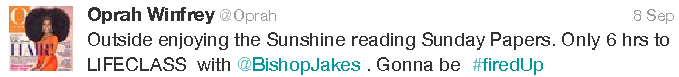
\includegraphics[width=8cm]{twitterTweetExample3-crop.pdf}}}
    \hfill
    \vfill
    \hfill
    \subfigure[]{\fbox{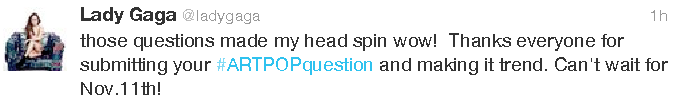
\includegraphics[width=8cm]{twitterTweetExample4-crop.pdf}}}
    \hfill
    \subfigure[]{\fbox{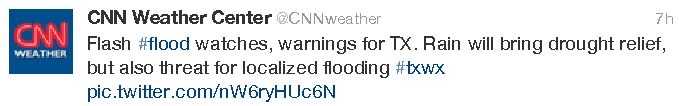
\includegraphics[width=8cm]{twitterTweetExample5-crop.pdf}}}
    \hfill
    \caption{Example tweets on twitter.com}
    \label{figTweetExample}
  }%
\end{figure}

Some example tweets on Twitter are included in Figure \ref{figTweetExample}.
Note how users both add hashtags to the end of a tweet as a summary of the message and emphasize important concepts words in the tweet by turning them into hashtags.
That is, hashtags are both intermixed within the words of the tweet and added to the end of the message.

These memory retrieval models will also be tested on tag use for StackOverflow posts.
StackOverflow is a question and answer site for computer programming where users ask programming-related questions and fellow members of the community provide answers.
A user with a programming-related question creates a post with their question and tags the post with a few specific programming-related tags. 
User-chosen tags on the StackOverflow site represent the primary topic of the question, such as a specific programming language, tool, software package, or framework.
Some example tags for StackOverflow are \emph{PHP}, \emph{Arrays}, \emph{MVC}, \emph{C\#}, and \emph{Common Lisp}.

\begin{figure}[!htbp]
  \scalebox{.8}{\resizebox{\linewidth}{!}{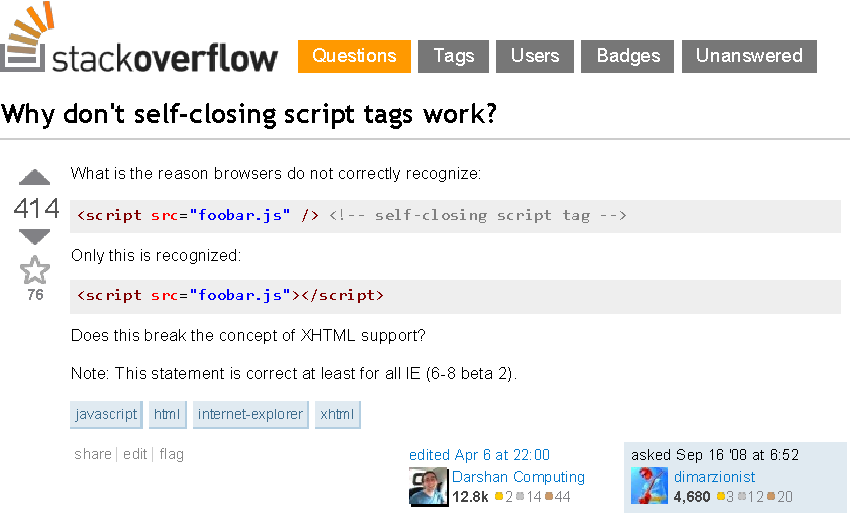
\includegraphics{stackoverflowPostExample1-crop.pdf}}}
  \caption{Example post on stackoverflow.com}
  \label{figSOExample}
\end{figure}

An example StackOverflow post is included in Figure \ref{figSOExample}.
The site requires that for each post the user must associate at least one tag with the post, and the average number of tags per post is around 3.
The author used 4 tags for this post: \emph{javascript}, \emph{html}, \emph{internet-explorer}, and \emph{xhtml}.

The StackOverflow and Twitter datasets were chosen because the human-created content between them is quite different, and I am interested in retrieval models that generalize across tasks.
However, they are also similar on several accounts:
Both domains have amassed large amounts of user-created content, users generate tags for posts when creating content on the site (hashtags for Twitter and tags for StackOverflow),
and the user data from the datasets are publicly available for analysis.

Also, studying user-based tag generation on these sites has relevant real-world application.
Models that can accurately predict the tags that users will generate on Twitter and StackOverflow can be used as the foundation for recommendations systems on these very popular sites.
These systems can also help newer users by recommending proper tags for their newest content.
On the StackOverflow site, for example, experts often subscribe to specific hashtags that interest them, and receive a daily digest of posts that are tagged with those hashtags.
Helping the user properly tag posts on StackOverflow ensures that right community sees the post, which greatly increases the chance that the question on the post will be answered quickly and correctly.
For Twitter, hashtags represent streams of information that are possibly interesting to the user.
Having a recommendation system that can suggest relevant hashtags to the user provides a way for the user to connect to and discover new information streams that interest them.

\subsubsection{Comparison Between ACT-R and Vector-Based Memory Systems}

ACT-R's declarative memory and vector-based memory systems are substantially different in their mathematical structure.
Nonetheless, both can successfully model classic behavioral patterns found in word pairing experiments (e.g., \cite{Rutledge2008} modeling the ``fan effect'').
I will extend the work done by \citeauthor{Rutledge2008} by formally comparing these two models on large-scale hashtag prediction tasks.
I will also replace the vector-based model used by \citeauthor{Rutledge2008} with an improved and simplified random-permutation model \parencite{Sahlgren2008}.

An advantage of vector-based models is that word order can be easily incorporated into the single co-occurrence representation \parencite{Jones2007}.
Word-order information on sites like Twitter may contain highly-predictive pieces of information, as it is likely that specific words immediately precede specific hashtags.
However, it is unclear and unexplored how word order can be represented in the ACT-R declarative memory theory.
I will explore how the word-order strength of vector-based models can be incorporated into the ACT-R theory when testing the models on hashtag prediction tasks.

ACT-R's declarative memory system places strong constraints on how a user's prior knowledge and experience influences the likelihood that a particular memory item is retrieved \parencite{Anderson2007}.
This decay rate equation formalizes how recency and frequency of hashtag use relate to the prior probability that a hashtag will be retrieved.
However, it is unexplored how a user's prior knowledge should influence retrieval for vector-based models.
I will explore how a user's prior knowledge influences the likelihood that a particular hashtag is chosen for both ACT-R's memory theory and vector-based models.

\subsubsection{Lifetime of a Hashtag for a Specific User}

Prior research has examined the growth and decay cycle of hashtag use across users \parencite{Tsur2012}.
However, much less is known about hashtag lifetime for individual users.
It may not necessarily follow that a hashtag's life cycle for individual users matches the life cycle across users.
Further, modeling a hashtag's life within users is much more applicable to hashtag prediction, since that model can be directly incorporated into a specific user's prior likelihood of hashtag use.
So I will characterize the hashtag growth and decay cycle for individual users.
The expectation is that this cycle will match ACT-R's decay rate used in the declarative memory system to compute a particular memory item's prior.

\subsubsection{User-Customized Hashtag Prediction}

The end goal of this work is to identify a memory retrieval model that can suggest relevant hashtags to users when they wish to retrieve one.
These hashtags should be customized to their specific interests and relevant to the content of the post that they are currently creating.
This will undoubtedly require a combination of two primary model components:
[1] A user's prior likelihood of choosing a particular hashtag, given their previous hashtag use, and [2] the likelihood that a particular hashtag is related to the context of the post being created. 

A user's prior hashtag use will be an essential model component for domains such as Twitter, where the number of possible hashtags is effectively infinite.
In these domains, the model can utilize a user's hashtag history as a way to prune the infinite space of possible hashtags, and generate a much smaller and more manageable set for prediction.
However, not only should the model properly take into account a user's prior hashtag use, but it should also generate new hashtag predictions when a user is most likely choosing a hashtag they have never used before.
The end goal is to have a model that can properly balance the user's tag history with the contextual cues in the post in order to generate an accurate prediction.

\section{Prior Research}

\subsection{ACT-R Declarative Memory Theory}

ACT-R \parencite{Anderson2007} is a cognitive architecture that formalizes how each cognitive process of the brain (e.g., memory, learning, visual and motor) interacts to produce behavior.
The declarative memory system is a component of that architecture that models the timing, learning, and forgetting processes that make up long-term declarative memory retrieval.
The equations that make up this system can be derived through a rational analysis of long-term memory retrieval.
That is, given the task of retrieving a chunk of information from long-term declarative memory,
the current context (i.e., external and internal environment state), and past experience (i.e., prior memories and exposure), 
what is the optimal behavior (i.e., the optimal chunk to retrieve from memory)?
Using Bayesian reasoning, each chunk of information in declarative memory can be assigned a prior likelihood of needing retrieval again, given the prior history of exposure to the chunk.
These chunk prior probabilities are then adjusted for the current context, so that the posterior probabilities represent the likelihood that a chunk is needed, given prior odds and adjusted by current environment state.

\subsubsection{ACT-R DM Model}

A formal description of the ACT-R Declarative Memory model is included in Table \ref{tabACTRModel}.

\begin{table}[!ht]
  \caption{ACT-R declarative memory model}
  \label{tabACTRModel}
  {\tabulinesep=1.2mm
    \begin{tabu}{ll}
      \hline
      Common Name &  Equation \\
      \hline
      Activation &	 	$A_{i} = B_{i} + \sum_{j \in c}^{} W_{j} S_{ji}$ \\
      Attentional Weight &	$W_{j} = \frac{W}{n}$ \\
      Base Level & 		$B_{i} = log \sum_{j=1}^{n} {t_{j}}^{-d}$ \\
      Constant Base Level &	$B_{i} = log \frac{p(i)}{p(\overline{i})}$ \\
      Strength of Association &	$S_{ji} = log \frac{p(i|j)}{p(i|\overline{j})} \approx log \frac{p(i|j)}{p(i)}$ \\
      Recall Probability &	$P_{i} = \left( 1 + e^{\frac{\tau - A_{i}}{s}} \right )^{-1}$ \\
      \hline
    \end{tabu}
  }
\end{table}

The total activation ($A_{i}$) for a chunk in declarative memory is a function of two components: base level activation ($B_{i}$) and strength of association ($S_{ji}$).
The recall probability ($P_{i})$ that a chunk will be retrieved from memory increases with total activation ($A_{i}$).

\subsubsection{Base-Level Activation}

Base-level activation reflects the log prior odds of needing an observed chunk again.
The primary way to calculate these log prior odds is to use the standard base level equation in Table \ref{tabACTRModel}.
This equation formalizes how log prior odds are a function of both frequency and recency of prior exposure to a particular chunk.
Chunks used more frequently (either through exposure or from a retrieval) are more likely to be needed for retrieval again.
However, as time progresses and a particular chunk is no longer used, the activation for that chunk decays.
In this way the standard base level equation formalizes the time dynamics of the retrieval system, where a chunk's base-level activation evolves over time, depending on its current frequency and recency of use.

For some domains it is reasonable to assume that the base-level activations of each chunk within a particular time window of interest are stable, and do not change within that window.
Programming-language popularity over the past few years is a reasonable example of this.
Although the popularity of various programming languages has certainly changed slightly over the past few years (e.g., Clojure's growth), it is not the case that the changes have been drastic.
C\#, Python, and Java are still a few of the most popular languages, Common Lisp has not gained or lost much ground in popularity over the past few years.

Further, if this is a reasonable assumption to make, it greatly simplifies the computation of the base-level activation for chunks, and can turn the computation into a tractable problem for large datasets.
In these time-constant domains, one can compute the log prior odds of needing each chunk directly as the log odds ratio of exposure to that chunk compared to exposure to all other chunks.
For example, if the StackOverflow tag \emph{PHP} has been used four times as often as the tag \emph{Common Lisp}, then the prior odds of needing \emph{PHP} again is $\frac{.8}{.2}=4$ times that of \emph{Common Lisp}.

\subsubsection{Strength of Association}

Strength of association ($S_{ji}$) reflects the amount of log odds adjustment to the activation of a chunk, given the current context (i.e., external environment and internal state).
Context for the StackOverflow domain for example is represented as each word in the title and body of a post.
Context for the Twitter domain are the words in a tweet.
Association strength between a chunk in memory and a single contextual element can be computed directly by calculating its context-adjusted odds ratio:
The likelihood a chunk occurred with the current context ($p(i|j)$) over the likelihood that the chunk occurred in any of the other contexts ($p(i|\overline{j})$).
For large datasets, the likelihood that a chunk occurs in any particular context reaches near-zero values ($p(j) \Rightarrow 0$).
So it can be assumed that the likelihood that a chunk occurs in any context but one ($p(i|\overline{j})$) is equivalent to the likelihood that a chunk occurs in any context ($p(i)$).
This assumption has been both mentioned and used when deriving the $S_{ji}$ equation \parencite{Anderson1989}, as well as in recent research working with large-scale datasets \parencite{Stanley2013}.

Using this assumption for large datasets ($S_{ji} = log \frac{p(i|j)}{p(i)}$), the interpretation of the context-adjusted odds ratio becomes much simpler.
If this ratio for a particular tag and context chunk is greater than one, then the log is positive, which means that this context has been observed more often with this tag than in general.
If this ratio is less than one, then the log is negative, which provides a negative adjustment of total activation since this context has been observed more often in general than with this particular tag.

\subsubsection{Connection to Pointwise Mutual Information}

Pointwise Mutual Information (PMI) is another co-occurrence index that measures strength of association between two terms \parencite{Farahat2004}.
It is based on the co-occurrence count between pair-wise observations of terms, similar to ACT-R's strength of association.
The PMI index is included in Equation \eqref{eqPMI}.

\begin{equation}
  \label{eqPMI}
  \mathit{PMI}(y,x) = log \frac{p(y|x)}{p(y)}
\end{equation}

Further, this PMI equation is identical to ACT-R's strength of association ($S_{ji}$) equation for large datasets.
Once the number of occurrences is large enough such that the probability of observing any particular contextual element ($p(x)$) is near zero, then ACT-R's strength of association index simplifies to the PMI equation.
That is, the PMI equation \emph{is} the simplified form of ACT-R's strength of association index ($S_{ji}$).

\subsubsection{Scaling the Equations}

The majority of tag-recommendation systems use some measure of word pair associations to compute the likelihood of a tag, given current context.
It is important that this measure scales well enough to handle the sheer volume of information present in online social media datasets.
Large-scale social media datasets such as StackOverflow and Twitter contain on the order of millions to hundreds of millions of unique word pair associations between terms and tags.
If one wants to capitalize on all of the information present in the database to build the most accurate measure of relatedness between words and tags, then the association measure used must scale to this large size.

ACT-R's strength of association ($S_{ji}$) and the equivalent pointwise mutual information index ($\mathit{PMI}_{ji}$) have been shown to scale well for large corpora.
\textcite{Douglass2010} implemented the large-scale version of $S_{ji}$ in Erlang.
The wall-clock time required for a declarative memory retrieval request scaled linearly with the size of declarative memory with this implementation.
Retrieval times were around one second with the largest declarative memory that contained over one million associations (co-occurrence pairs).

The SNIF-ACT framework \parencites{Fu2007,Pirolli2003} is also based on the large-scale version of $S_{ji}$, and scaled well when working with a large-scale search query database for internet search.

As one of the largest tests, \textcite{Farahat2004} used the PMI index based on a 118GB local database of 10 million pages of the Stanford WebBase Project.
So this implementation did not fit completely in RAM, but a spinning-disk database implementation still scaled well enough for reasonably fast retrieval times for $\mathit{PMI}_{ji}$ values.

\subsection{Latent Semantic Analysis Memory Theory}

Latent Semantic Analysis \parencite{Landauer1997} (LSA) is a technique that has mathematical roots in factor analysis and also measures strength of association between two terms.
The process starts with a set of N documents.
A word by document co-occurrence matrix is built by counting the number of times each word appears in each document.
The dimensionality of the full word frequency co-occurrence matrix is then reduced, while maintaining as much of the variance in the original full matrix as possible.
This process is similar to how factor analysis takes a data table and finds the most efficient way to represent that data with as few dimensions as possible.
The strength of association between two words is measured by the cosine of the two word vectors across the reduced dimension space.

Usually information is lost when the data are restructured into a smaller set of latent dimensions.
However, it was shown that this process actually improves prediction and reduces noise by allowing the frequency count of highly similar concepts (words) to be pooled together and represented by a single dimension.
\textcite{Landauer1997} tested the LSA model on the Test of English as a Foreign Language (TOEFL) task of choosing the best of four possible synonyms to a target word.
Model results were on par with a large sample of applicants to american universities from non-English speaking countries (64.4\% compared to 64.5\%).
Model performance also improved when the original dimensionality of the data was reduced, but only up to a point.
Afterwards further reductions in the dimensionality of the data began to degrade performance.

\subsubsection{Singular Value Decomposition}

LSA uses the Singular Value Decomposition process to reduce the dimensionality of the word by document co-occurrence matrix.
The technique attempts to maximize the amount of variability in the data left after forcing the original dimensionality of the data to be reduced.
The best way to remove a dimension while maintaining the most variability is to look for words with highly-similar co-occurrence patterns and deduce that these words represent the same concept.
For example, synonyms such as \emph{\#photograph} and \emph{\#photo} would appear interchangeably across documents, so these terms would be collapsed to a single dimension and frequency counts would be pooled.
By pooling co-occurrence counts the model is able to generate better predictions with less data.

\subsubsection{Word Order}

Although the LSA model has been shown to perform well as a way to measure similarity between two terms, one of the main criticisms is that it is a ``bag of words'' model.
This means that the model does not account for or pay attention to word order when building the base word by document matrix or consequently, when performing the SVD dimension reduction.
Other models that can account for word order have been shown to perform better than ``bag of words'' models on tasks that do not even appear to require grammatical structure such as word order to do well.
For example, \textcite{Jones2007} compared a vector-based model called BEAGLE directly to LSA, training and testing both models on the same corpus used in \textcite{Landauer1997}.
The context-only BEAGLE model (no word order) performed nearly equivalent to the LSA model at the task (55.6\% vs. 55.3\%).
However, even in a multiple-choice domain where the task is to identify synonyms (very little grammatical structure in the task), adding word order when training the model improved task performance to 57.5\%.
It seems reasonable to expect that task performance will improve much more on tasks where word order is used (e.g., generating a hashtag in the middle of a sentence when composing a tweet).

\subsubsection{Scaling Issues}

Another issue with LSA is that the SVD matrix decomposition technique is computationally very expensive.
As the size of the original word by document matrix increases, the SVD computation becomes more and more time consuming.
If the domains where LSA is applied contained small enough datasets where SVD computation could be computed in a reasonable amount of time, then this would not be much of a concern.
However, with large-scale human-created datasets such as Twitter, Stackoverflow, and Wikipedia, the total size of the dataset far exceeds the maximum size that can even be computed by an LSA approach.
\textcite{Budiu2007} used the first six million pages of the Stanford WebBase corpus to compare performance between LSA and PMI on the TOEFL, and the LSA model could not be implemented with this size training dataset.
Instead, they compared the measures on the TOEFL by training on the smaller Touchstone Applied Science Associates (TASA) corpus created from \num{60527} samples of text from high school to early college textbooks.
This is one of the available corpora on the LSA website and is aimed to summarize the general reading up to the 1st year of college \parencite{Budiu2007}.

When \textcite{Budiu2007} compared the simpler PMI (i.e., $S_{ji}$) measure to LSA on smaller TASA-corpus-size datasets, LSA performed much better (23\% vs. 60\%).
This was one of the primary motivating reasons that LSA was developed in the first place, since reduced dimensionality model out-performed the full dimensionality model on TASA-sized datasets.
However, once the dataset surpasses in size what is computationally feasible with LSA, the much simpler PMI measure can still be computed, and the performance for PMI becomes on par and even surpasses that of LSA.
\textcite{Budiu2007} also trained the PMI measure on the much larger Stanford WebBase corpus and tested the measure on the TOEFL.
This PMI model increased accuracy from 23\% to 51\% when training the dataset on the smaller TASA compared to the larger Stanford dataset.
Further, when \textcite{Turney2001} trained the PMI measure on the even larger AltaVista index of 350 million webpages, the accuracy on the TOEFL increased to 73.75\%, which is 10\% higher than the TASA-trained LSA.
This suggests that simpler models may be preferred to more complex (yet more accurate) models in large-scale domains, since the simpler models scale and can utilize all available information to generate predictions.

\subsubsection{Cost of Incremental Updating}

Another issue with LSA is that adding additional observations to an already-computed reduced representation requires rerunning the SVD \parencite{Farahat2004}.
Since computing the SVD is the most computationally-expensive operation with LSA, it is difficult to see how LSA could be implemented in incremental domains where information is periodically added.
For Twitter and StackOverflow, it might certainly be useful to update the strength of association representation when new information arrives, especially for Twitter, where hashtag use and news content change rapidly.

\subsection{Vector-Based Memory Systems}

``Holographic'' memory systems \parencite{Plate1995} or vector-based memory systems represent a concept (i.e., chunk) as a vector.
The representation of the concept is distributed across all elements of the vector.
This is somewhat similar to taking a column (i.e., a tag) on a word co-occurrence matrix and viewing the distribution of co-occurrence counts across the rows in the column as the representation of that concept.
However, vector-based memory systems represent information in a much more compact way than a full word co-occurrence matrix.

For vector-based systems, each word is represented by an environment vector $e_{i}$ that is nearly orthogonal to all other words' environment vectors.
The number of dimensions for these vectors is much less than the number of rows in a full word co-occurrence matrix, which is how vector-based systems represent information in a much more compact space.
Paired with each environment vector ($e_{i}$) is a memory vector ($m_{i}$) that contains the summed representation of all other environment vectors that have co-occurred with that $e_{i}$ environment vector.
These memory vectors can contain environment vectors from position-independent word co-occurrence information ($c_{i}$) and word order information ($o_{i}$), which can be combined into a single representation ($m_{i}$).
Over time, memory vectors accumulate a distributed representation of the most common environment vectors that co-occurred with them.

\subsubsection{Retrieval Process}

Retrieving the most likely chunk given context can be done in two ways: decoding and resonance \parencite{Jones2007}.
Decoding takes the memory vector for context and decodes it back into an environment vector.
The cosine between that decoded environment vector and all other environment vectors is computed and ranked, and the chunk with the environment vector with the highest cosine is retrieved.

Resonance is the opposite retrieval process, where a memory vector is created from the context, and then that context memory vector is compared to all memory vectors.
For example, assume that a user has written the word ``zend'' in a post, and she wants to assign a tag for the post.
``zend'' has co-occurred with the tag \emph{PHP} many times previously, so the unordered memory vector for ``PHP'' ($c_{\mathit{PHP}}$) contains the unordered environment vector for \emph{zend} ($e_{zend}$).
To determine the most correlated memory vector with context, a memory vector is created from the current context ($e_{zend}$).
The cosine between that context memory vector and the memory vector for \emph{PHP} will be high, since the \emph{PHP} memory vector ($c_{\mathit{PHP}}$) often contains the context environment vector ($e_{zend}$).
Since the cosine is high, the tag \emph{PHP} will most likely be returned as the vector that resonates highest with the current context.

The resonance and decoding processes are inversions of each other.
Usually both resonance and decoding will return very similar rank orderings of most likely chunks given context.
\textcite{Jones2007} recommends averaging the cosine values returned from each process for each chunk, and then rank ordering those averages to determine the chunk to retrieve.
However, decoding does require an additional decoding step that resonance does not require, and depending on the decoding operation, this step may be computationally expensive.

\subsubsection{Addressing Word Order}

One of the strengths of vector-based systems is that word order can naturally be represented alongside word co-occurrence in these distributed representations.
Representing word order is a case where both the encoding and decoding operations are applied.
As a motivating example, say that one wants to encode the first and second words immediately preceding a hashtag in a tweet.
Simply counting co-occurrences of the two immediately-preceding words and hashtags does not include the order information of the words in the representation.
With this representation, it would be impossible to tell the difference between 1-back words that immediately preceded the hashtag, and 2-back words that occurred just prior to these 1-back words.
Order information is lost if a simply co-occurrence counting technique is used.

With vector-based systems, order information is included by creating an environment vector ($e_{bind(i,\Phi)}$) that is a function of environment vectors for both the word ($e_{i}$) and location ($\Phi$).
This function has the useful property that the resulting environment vector and the location vector can be inverted to return the original word's environment vector.
Circular convolution and inverse circular convolution (i.e., circular correlation) are used by \textcite{Plate1995} and \textcite{Jones2007} to implement these operations.
This allows for retrieval requests such as ``playing \#$\Phi$'', ``just read \#$\Phi$'', and ``vector-based $\Phi$ systems''.

For example, suppose that a retrieval request is made for ``martin $\Phi$'' given that the model was trained on the TASA corpus.
Within this corpus, the phrase ``martin luther'' often occurred.
When this occurs, the word-order memory vector for martin ($o_{martin}$) will be updated by convolving a 1-back location vector with luther ($o_{martin} = o_{martin'} + \Phi * e_{luther}$).
Also, the word-order memory vector for luther ($o_{luther}$) will be updated by convolving martin with and a 1-forward location vector ($o_{luther} = o_{luther'} + e_{martin} * \Phi$).
The retrieval request for ``martin $\Phi$'' can be done in two ways: through decoding or resonance.

Using decoding, the word-order memory vector for martin is deconvolved to the right ($o_{martin} \circledast \Phi$) which returns the environment vector for luther ($e_{luther}$).
Using resonance, a memory vector for ``martin $\Phi$'' is constructed ($e_{martin} * \Phi$), which correlates highest with the word-order memory vector for luther ($o_{luther}$).
Either way, luther is returned as the most likely term to match the phrase ``martin $\Phi$''.

New vectors generated by circular convolution are uncorrelated with all other environment vectors and have the same length.
This allows the word order information and unordered context information for a chunk to be aggregated and represented in the same memory vector.
Quite simply, the different types of memory vectors can be summed to create a single memory vector representation for each chunk (i.e., $m_{i} = c_{i} + o_{i}$).

\subsubsection{Addressing Scalability}

Vector-based representations compute chunk likelihoods by performing a correlation operation directly on the memory vectors.
Each memory vector can be thought of as a column on a context word by tag co-occurrence matrix used for a Bayesian representation.
Further, the number of rows for a vector-based representation are fixed and set much smaller than the number of rows in the full word by tag co-occurrence matrix.
Since Bayesian representations have been shown to scale to over hundreds of millions of word by tag co-occurrences \parencite{Stanley2013}, the compressed vector-based representations should scale as well or better.

\subsubsection{BEAGLE}

\textcite{Jones2007} created the BEAGLE vector-based memory representation.
Each memory vector ($m_{i}$) is a summed representation of unordered and ordered word co-occurrences ($c_{i} + o_{i}$).
This model uses circular convolution and circular correlation as a way to encode and decode word order.
BEAGLE performed similar to LSA when trained on the TASA and tested on the TOEFL (55.6\% compared to 55.3\%).
Also, BEAGLE with unordered context and word order was more correlated to the WordNet synonym database than LSA (-.311 compared to -.165).
Further, it was shown that incorporating word-order information into the same representation resulted in minimal data loss (less than 1 percent of total predictive variance).
This model provided an efficient algorithm for using a single representation for unordered and ordered information that showed performance similar to if not better than LSA.

\subsubsection{Random Permutation Model}

In order to represent word order information, a function must be used that converts an environment vector for a set of words and positions (e.g., ``stack $\Phi$'') into a new uncorrelated environment vector.
The BEAGLE model uses circular convolution and circular correlation as the encoding and decoding operations.
However, that is certainly not the only operation that can generate new uncorrelated vectors from a set of memory vectors and positions.
\textcite{Sahlgren2008} used a much simpler random permutation method for this operation.

A formal description of the random permutation model in \textcite{Sahlgren2008} is included in Table \ref{tabRandPermModel}.

\begin{table}[!ht]
  \caption{Random permutation model}
  \label{tabRandPermModel}
  {\tabulinesep=1.2mm
    \begin{tabu}{ll}
      \hline
      Common Name &  Equation \\
      \hline
      Activation &		$A_{i} = r(m_{C},m_{i})$ \\
      Memory Vector &		$m_{i} = \sum_{i \in all past} c_{i} + \sum_{i \in all past} \sum_{l \in locations} o_{i,l}$ \\
      Unordered Context &	$c_{i} = e_{i}$ \\
      Ordered Context &		$o_{i,l} = e_{i^{-l}}$ \\
      Context Memory Vector &	$m_{C} = \sum_{i \in C} c_{i} + \sum_{i \in C} \sum_{l \in locations} o_{i,l}$ \\
      Environment Vector & 	$e_{i} = rand$ \\
      \hline
    \end{tabu}
  }
\end{table}

With random permutations, each word environment vector ($e_{i}$) is a large sparse vector of zeros with a few one and negative one values in random locations. 
In order to create a new environment vector for a word that preceded another word in a sentence, that word's environment vector is shifted to the left one position.
This produces a new environment vector ($e_{i^{-1}}$) for the combination of the word and the position that is uncorrelated with the original word's environment vector and all other environment vectors.

For example, suppose that the words ``stack overflow'' appear in a sentence, and I want to represent that ``stack'' preceded the word ``overflow''.
The ``stack'' environment vector ($e_{stack}$) is shifted one to the left, producing an environment vector for ``stack'' preceding a word ($e_{stack^{-1}}$).
That environment vector is then added to the memory vector for ``overflow'' ($m_{overflow} = m_{overflow'} + e_{stack^{-1}}$), so that ``overflow'' remembers that ``stack'' has preceded it in a sentence.

A resonance retrieval for a word following ``stack'' (``stack $\Phi$'') is done by creating a memory vector out of all information in context.
In this case, assume only a single piece of order information is available, that ``stack'' precedes the word to retrieve.
So the memory vector for context is the environment vector for one-back ``stack'' ($m_{C} = e_{stack^{-1}}$).
The memory vector for ``overflow'' ($m_{overflow}$) will be correlated the highest with this context vector ($m_{C}$) since ``overflow'' contains this vector.

\subsubsection{Comparison between BEAGLE and Random Permutations}

Random permutations uses one of simplest permutations possible to create a new environment vector.
This operation is much less costly than circular convolution used by the BEAGLE model, which allows random permutations to scale better and handle larger datasets.
Further, even though random permutations is a simpler representation than BEAGLE, it also performs better when trained on the same sized corpus. 

\textcite{Recchia2010} found that random permutations could use smaller vectors than circular convolution approaches (e.g., BEAGLE) to produce equivalent performance (better compression),
and also scale to larger datasets (better computational efficiency).
The vector length by performance tradeoff was tested on a simple paired associative retrieval task. 
Retrieval accuracy for the random-permutation vector-based models remained high relative to the circular convolution model even after reducing each environment vector's length from \num{2048} to \num{1024}.
This indicates that vector-based representations using random permutations compress better than those using circular convolution.

To test computational efficiency, each model was trained on a subset of the Wikipedia corpus, and tested on the Test of English as a Foreign Language (TOEFL) assessment (among other tasks).
The random-permutation model was trained on \num{2.33} GB corpus.
The BEAGLE model was unable to train on a corpus this large, so both models were also trained on an additional \num{35} MB subset of the Wikipedia corpus.
The random permutation model performed as well or slightly better than the BEAGLE model when trained on the smaller corpus.
The model's performance also significantly improved when trained on the much larger corpus that was computationally intractable for the BEAGLE model.
These results make a strong case to favor random-permutations over circular convolution when implementing vector-based memory representations.

\subsubsection{Connection to LSA}

Both random permutations and LSA calculate word similarity on a reduced matrix.
For LSA, the original word by document matrix is compressed to a factor by document matrix and the number of factors are much less than the number of words.
For the StackOverflow and Twitter datasets, the number of documents are the number of different tags.

For random permutations, each tag is represented by a compressed vector with a length much less than the number of words.
Note that if the length of a word's environment vector was the number of unique words, then each word could be represented by associating it with a particular row in the column vector.
If done in this way, building a matrix of all words' environment vectors by tags would recover the original word by document matrix \parencite{Kanerva2000}.
However, each word's environment vector is compressed using a length much less than the number of unique words and represented by using a combination of a few one and negative one values at a unique combination of positions. 

Information is lost with this compression in both cases: by starting with a compressed representation with random permutations or by reducing to a compressed representation with LSA.
However, the way that the compression works in these two cases is not the same.
LSA uses SVD to find words that have highly correlated tag occurrence distributions (i.e., latent concepts), and then pools those co-occurrence counts into a single dimension.
A vector-based approach like BEAGLE or random permutations essentially randomizes the mapping of the words on the reduced set of dimensions, and does not take into account word similarity when generating the mapping.
Nonetheless, random permutations have been shown to perform similar to if not better than LSA when trained on the TASA and tested on the TOEFL \parencites{Sahlgren2008,Jones2007}.

This is a counterintuitive result.
It seems plausible that an SVD technique that takes into account word similarity when reducing the matrix should generate a reduced matrix that has more information than a randomly-compressed matrix.
This does not seem to be the case in testing however, as vector-based approaches like BEAGLE and random permutations perform just as well as the LSA when trained and tested on similar datasets.
Nonetheless, it has been suggested to perform an SVD reduction technique on a compressed random-permutation vector \parencite{Kanerva2000}.
This approach might be worth investigating, as it would reduce computational requirements even further, and possibly improve performance by pooling co-occurrence counts from latent topics together.

\subsection{Comparison of Vector-Based Models and ACT-R}

Vector-based models can be thought of as a compressed representation of the full co-occurrence matrix used for the ACT-R declarative memory system.
Each model computes an activation for each word to retrieve, given context and (for ACT-R's Bayesian model) prior knowledge.
Since both models produce activations for each chunk, one can be swapped out for another and used as the declarative memory component of the ACT-R infrastructure.
For example, \textcite{Rutledge2007} used a variant of the BEAGLE vector-based model as the DM component of ACT-R.
\textcite{Rutledge2008} showed that an ACT-R theory with a vector-based memory system can successfully model the fan effect, which is a psychological phenomena that ACT-R's current Bayesian DM system can model as well.

\subsubsection{Base-Level Activation}

Vector-based models and ACT-R's current Bayesian DM model are not identical however, and these differences need to be addressed in order to better evaluate the benefits of one over the other.
For example, the frequency and recency of retrievals for each chunk are not currently used for vector-based models when calculating activation.
More recent tweets on a news site like Twitter should be more relevant, for example.
\textcite{Efron2011} tested this claim by evaluating a set of query likelihood models on returning relevant Twitter tweets from search queries.
They showed that a model incorporating recency information of the tweet produced more relevant results than models that did not pay attention to this information.

ACT-R's Bayesian model has a strong theory with respect to recency and frequency information.
It uses this information to calculate a chunk's prior activation (i.e., prior likelihood of being needed again, independent of current context).
Vector-based models compute activation based entirely on context, so chunks that resonate with context will be retrieved, irrespective to the frequency and recency of use of that chunk.
ACT-R's prior activation can also be computed for each user, so that hashtags that have been used frequently and recently for a particular user are rated with higher activation.
This type of information on a user's prior behavior is not being utilized with vector-based models currently.
It may certainly be the case that vector-based models can be modified to incorporate base-level activation, and this idea will be pursued with this research.

\subsubsection{Word Order}

One strength of a vector-based model over ACT-R's Bayesian DM model is that word order can be naturally represented alongside unordered co-occurrence information.
With the ACT-R model, for example, it is unclear how to represent that a particular word appeared just before a hashtag. 
It may be that multiple co-occurrence matrices must be used to represent word-order co-occurrences and unordered co-occurrences separately.
However, it would be more parsimonious if these matrices could be combined into a single matrix representation, much like how this information is combined for vector-based models.

\subsubsection{Activation Calculation}

Vector-based and LSA retrieval models calculate chunk activation by correlating a representation of the current context with each memory item.
Bayesian retrieval models like ACT-R calculate activation by computing each chunk's posterior odd adjustment likelihood, given the context.
These two computations are certainly not equivalent, even though they are most likely correlated with one another.
It may be interesting to explore how model performance changes when one calculation is swapped out for another.
For example, a vector-based model could generate a compressed (reduced dimension) co-occurrence matrix, and then Bayesian calculations could be performed on that matrix to compute adjusted odd likelihoods.
Alternatively, a vector representation of the current context could be correlated with each column in a full co-occurrence matrix.
It is unlikely that the latter technique will improve performance, as \textcite{Landauer1997} has shown that performing correlations on uncompressed co-occurrence matrices does not perform well.
But it may be the case that using Bayesian computation on a compressed vector-based model improves performance.

\subsection{Recommendation Systems}

A model that predicts a user-chosen hashtag is a specific type of a recommendation system.
These general recommendation systems have grown in need with the growth of the web.
Users on a site need quick access to specific pieces of information, and the site contains much more information than they can process or care about.
Recommendation systems are used to tailor the information presented to what is most relevant to the user \parencite{Pazzani2007}.

\subsubsection{The Netflix Prize}

The Netflix Prize \parencite{Bennett2007} is an example of a recommendation system where prior user behavior and current context was used to present the most relevant information to the user.
Netflix is an online-subscription service where users can stream their favorite television episodes and movies.
Each user of the site is only interested in a small portion of the entire library of content that Netflix provides.
In order to provide a high-quality user experience on the site, Netflix created a content-recommendation service.
This tool recommends to the user movies and television episodes that most likely match their specific interests.

Netflix wanted to improve the accuracy of their recommendation system, so they held a competition where teams could try to improve on the accuracy of the service.
The winning team utilized a statistical model that performed a type of factor analysis to identify important dimensions in the data (e.g., drama, action, cult classic) and place values for each user along each dimension. 
This method used prior user behavior to classify a user along the dimensions of the reduced space, and current user behavior (e.g., just watched) to understand what they were interested in watching at that moment.
By using a factor-analysis technique and combining these indicators, the model improved on Netflix's original recommendation system by 10\%.

\subsubsection{Recommending Followers on Twitter}

Recommendation systems based on the content of user-created posts have been successful in recommending people on Twitter for a user to follow.
\textcite{Hannon2010} built a Twitter follower recommendation system by creating a profile of each user based on the words they used in previous posts.
The recommendation system would then suggest other Twitter users to follow that had similar profiles to a particular user.
The profiles were created by generating a word frequency matrix of words by (user + followers + followees), and then providing that matrix as input into the Lucene text search engine framework.

Lucene \parencite{McCandless2010} is a commonly-used open-source software tool that measures the similarity between a query and candidate documents in a database.
It uses the term frequency---inverse document frequency co-occurrence measure to quantify the similarity between a word in the query and a possible document to retrieve.

When \citeauthor{Hannon2010}'s system recommended a set of individuals for a user to follow, it collected all of the words used in posts from that user, constructed a search query, and provided that query to Lucene.
Lucene then returned the most likely users that share similar words in posts within their Twitter network with the words provided in the query.
Using this simple technique based on a standard text search engine allowed the recommendation system to accurately predict the people that a particular user follows at 25\% accuracy.

\subsubsection{Hashtags for Recommendation Systems}

\textcite{Efron2010} showed how hashtags might be used as a type of recommendation system for Twitter.
Users constructed a query of text that represented a search for a topic that they were interested in.
The system then retrieved the most likely hashtags that were associated with that search query.
The model is based on building a word co-occurrence matrix of words by hashtags, and then uses that matrix to assign a similarity score for each hashtag when provided with a search query.
Participants graded how relevant the hashtags returned were to each search query.
The results suggest that hashtags contain useful information that help classify the gist of a post. 
Although this model does not predict the specific hashtags used when composing a tweet, a model like this could certainly be tailored for that purpose.

\subsection{Hashtag Prediction}

Recommendation models that attempt to predict a user's chosen hashtag have recently been created and tested for a few social media sites.
Google has even deployed a hashtag-recommendation model to help users properly tag posts on their Google+ social media site \parencite{GoogleKeynote2013}.
A tag-suggestion tool has also been deployed for the \url{http://tex.stackexchange.org} and \url{http://superuser.com} StackExchange sites.
Models for Twitter and StackOverflow have been proposed and tested, but none have yet been deployed.

\subsubsection{StackOverflow}

\textcite{Kuo2011} was the first to model tag use for StackOverflow posts.
His set of models were originally designed for next-word prediction for large text document collections.
In order to structure the models to work for StackOverflow tag prediction, the models would request the most-likely next word after a user created a post, and restrict the space of possible words to only tags.
He tested the set of next-word prediction models to generate predictions for the most likely tags that a user would choose when asking a question on the site.
Interestingly, the Bayesian co-occurrence model outperformed the more complicated and computationally expensive Singular Value Decomposition and K-nearest-neighbors models.
This Bayesian model can accurately predict a user-chosen tag at 47\% accuracy.

% ref: http://tex.stackexchange.com/questions/53513/hyperref-token-not-allowed
\paragraph{\texorpdfstring{\textcite{Stanley2013}}{Stanley2013}'s ACT-R DM Model for StackOverflow}

\textcite{Stanley2013} also modeled a user's chosen tags for a post on the StackOverflow site.
They modified the standard ACT-R model in Table \ref{tabACTRModel} in order to more accurately predict tag use on StackOverflow.
A formal description of the modified ACT-R Bayesian model is included in Table \ref{tabModACTRModel}.

\begin{table}[!ht]
  \caption{\citeauthor{Stanley2013}'s StackOverflow tag prediction model}
  \label{tabModACTRModel}
  {\tabulinesep=1.2mm
    \begin{tabu}{ll}
      \hline
      Common Name &  Equation \\
      \hline
      Activation & 		$A_{i} = B_{i} + \sum_{j\in T}^{ } W_{j} S_{ji} + \sum_{j\in B}^{ } W_{j} S_{ji} - O$ \\
      Base Level & 		$B_{i} = log \frac{p_{i}}{1-p_{i}}$ \\
      Strength Assoc. &		$S_{ji} = log \frac{p(i|j)}{p(i))} = log \frac{NN_{ji}}{N_{Row}(j)N_{Col}(i)}$ \\
      Co-occurrence &		$N_{ji} = \sum_{}^{}{observed_{ji}}$ \\
      Observations &		$N = \sum_{}^{}{\sum_{}^{}{N_{ji}}}$ \\
      Attentional Weight& 	$W_{j} = W \frac{E_{j}} {\sum_{}^{} {E_{j}}} $ \\
      Scaled Entropy & 		$E_{j} = 1-\frac{H_{j}}{H_{max}}$ \\
      Entropy & 		$H_{j} = -\sum_{i=1}^{N}p(i|j)log\left (  p(i|j) \right )$ \\
      Offset & 			$O = \frac{1}{5}\sum_{i\in top 5}^{ } A_{i}$ \\
      \hline
    \end{tabu}
  }
\end{table}

The activation of each tag ($A_{i}$) is a function of four components:
That tag's base level activation ($B_{i}$), contextual activation for the words in the title, activation for words in the body, and an offset term ($O$).
This model has been modified from the standard ACT-R model (Table \ref{tabACTRModel}) in three ways:
Two separate contextual components were used (words in title and body of post), an offset term was added, and an entropy measure was used to compute the attentional weight ($W_{j}$).

The offset term was added to normalize the mean activation across retrievals.
This allowed the use of a logistic regression statistical technique to calibrate the weights for each of the terms.
The title and body contextual components were separated since it seemed plausible that the words in the title would be better predictors of the tag used than the words in the body.
It turned out that the words in the body were a better predictor of tag use \parencite{Stanley2013}, most likely because there are many more words in the body than the title of the post.
The entropy measure was used to compute the attentional weight for two reasons:
Stop words could be statistically derived and attenuated in the analysis, and more predictive words of some tag (e.g., the word ``PHP'' in a post) were given higher weight.
Using an entropy measure (as opposed to weighting each word equally in the post) for the attentional weight term allows the model to allocate limited attentional resources ($W$) to important contextual elements.

\paragraph{Comparison Between \citeauthor{Kuo2011}'s and \citeauthor{Stanley2013}'s Models}

Several modifications to \textcite{Stanley2013}'s model were made from the standard Bayesian ACT-R declarative memory theory,
so it was more sophisticated than the standard ACT-R model and the model used by \textcite{Kuo2011}.
\citeauthor{Stanley2013} used a data-driven entropy weighting measure to attenuate low-predictor words and increase the weighting of high-predictor words in the body and title of a post.
An offset term was also included which leveled the model's overall prediction for each post and enabled the use of a logistic regression statistical technique to calibrate the model's parameters.
A separate model component was used for the words in the body and title of the post, and it was unclear if \citeauthor{Kuo2011} used the words in the body of the post for his models.

\citeauthor{Stanley2013}'s model also scaled much better than \citeauthor{Kuo2011}'s co-occurrence model. 
Because of this, 100 times more posts were used to build the co-occurrence matrix (\num{1000000} versus \num{10000}), which significantly increased the model's performance.
After including the modifications and scaling up the model, the model can successfully predict a user's tag for a post at 65\% accuracy.

It is interesting that in both research papers the best performing model was based on a Bayesian co-occurrence framework, since that is precisely the framework from which ACT-R's declarative memory system is based.
This suggests that more cognitively-plausible memory retrieval models may outperform more general machine-learning approaches in this particular environment
(i.e., when predicting the user-chosen tags for human-created content on social media sites).

\subsubsection{StackExchange}

A tag suggestion tool has been deployed for the \url{http://tex.stackexchange.org} \parencite{LatexTags2013} and \url{http://superuser.com} \parencite{SuperUserTags2013} StackExchange sites.
Latex, SuperUser, and StackOverflow are all part of the broader StackExchange network of question and answer sites, and they provide the same user interface and workflow when asking questions.
For the two sites where a tag suggestion tool has been deployed, once a user has created a question, suggested tags appear just below the text field where the user types the tags to associate with the question.
The post author is not forced to use the suggested tags, and is free to choose tags from them or tags not represented in the suggested set.
An example of the interface for a created post on the SuperUser site is included in Figure \ref{figSuperUserSuggestion}.

\begin{figure}[!htbp]
  \scalebox{.9}{\resizebox{\linewidth}{!}{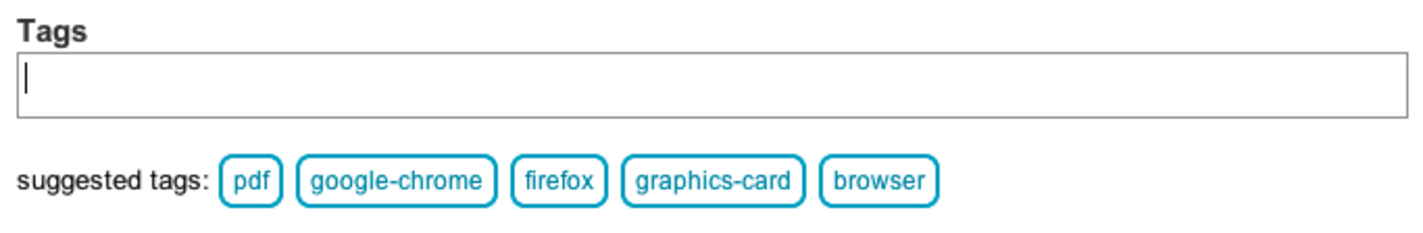
\includegraphics{superUserTagSuggestion-crop.pdf}}}
  \caption{Example of tag suggestions when creating a post on the SuperUser site}
  \label{figSuperUserSuggestion}
\end{figure}

The exact tag-recommendation algorithm used for the Latex and SuperUser sites is not publicized.
StackExchange appears to be using something more sophisticated than simply looking for words in the title and body of the post that are tags, as the algorithm has not yet been deployed for the busiest StackOverflow site.
The Latex and SuperUser sites are not nearly as popular as StackOverflow currently.
The sites have roughly \num{50000} and \num{189000} questions respectively compared to \num{5000000} questions on StackOverflow.

So it stands to reason that the algorithm is relatively complex, and there are possible scaling and efficiency concerns with the algorithm's implementation.
Or it is also possible that StackExchange decided to try out a tag recommendation system on a few of their smaller sites first, before deploying this type of system on their most popular StackOverflow site.
Nonetheless, it is encouraging that StackExchange finds tag recommendation models beneficial to the user and has started to add them to their question and answer sites. 

\subsubsection{Google+}

The hashtag recommendation system deployed for the Google+ microblogging service is probably the most ambitious model of user-created hashtags to date \parencite{GoogleKeynote2013}.
The user interface for this recommendation system for an example Google+ post is shown in Figure \ref{figGoogle+Hashtags}.

\begin{figure}[!htbp]
  \scalebox{.4}{\resizebox{\linewidth}{!}{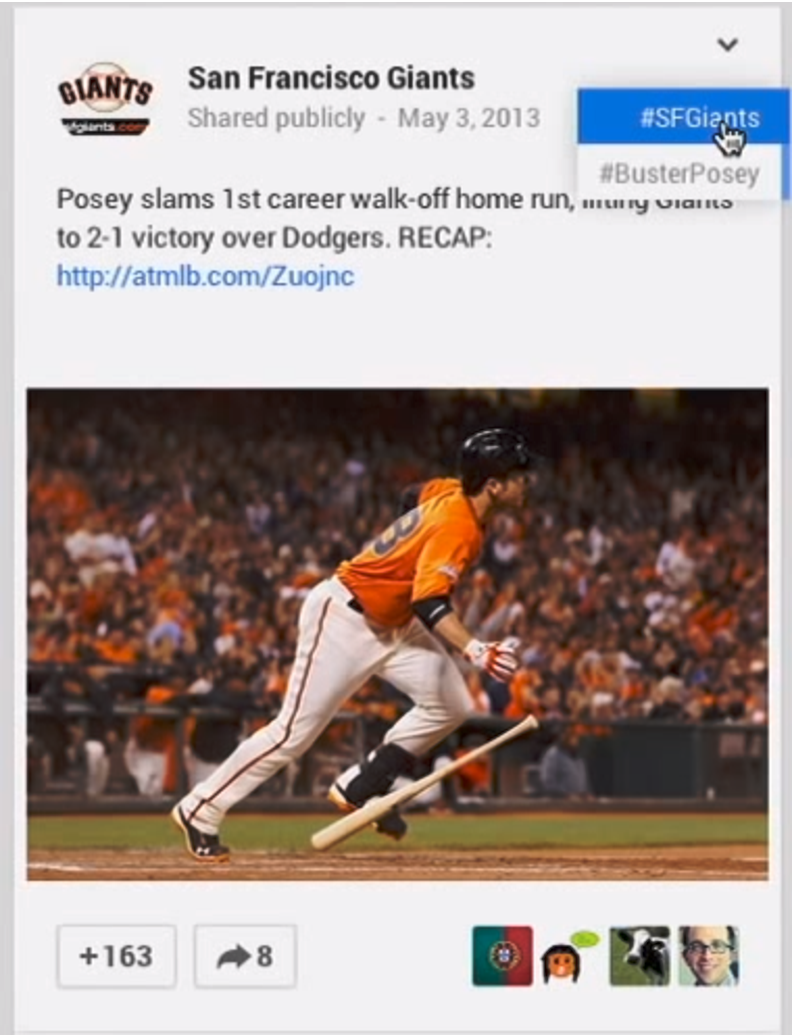
\includegraphics{google+HashtagExample-crop.pdf}}}
  \caption{Example post on Google+}
  \label{figGoogle+Hashtags}
\end{figure}

The workflow and user interface provided for recommending hashtags for Google+ is similar to how a hashtag recommendation system for Twitter might look.
When generating content on Google+, the system automatically associates the most likely relevant hashtags with that post.
For the example in Figure \ref{figGoogle+Hashtags}, the system recommended \emph{\#SFGiants} and \emph{\#BusterPosey} as hashtags for the user-created post.
The user is free to remove any or all of the tags that the system has associated with the post, and can also use tags that were not included in the recommended set.

Google+'s tag-recommendation algorithm is not publicized, but it appears to be rather sophisticated.
Looking at the example post in Figure \ref{figGoogle+Hashtags}, \emph{\#BusterPosey} is suggested without having that specific word in the post.
Also \textcite{GoogleKeynote2013} mentioned that the algorithm uses Google's sophisticated image recognition software to suggest hashtags for images that are included in the post (e.g., \emph{\#EiffelTower}),
even when the post does not have any keywords to provide additional context.

Google is apparently highly confident in the accuracy of their system.
On the Latex site, the user interface provides subdued suggestions to the user, but requires the user to explicitly choose each tag he/she wants to associated with the post.
For Google+, the user interface automatically tags a user's post, and then requires the user to explicitly change those tags if he/she wants to use a different set.
If tag accuracy is high enough, the Google+ technique is certainly favorable since the user does not have to spend time figuring out which tags best represent this post.
However, if the model makes even just a few errors, users may become annoyed and frustrated with the recommendation system since they will have to explicitly correct it every time they generate a post.

\subsubsection{Twitter}

Several hashtag recommendation models for Twitter have been developed recently.
One of the first models used a Bayesian co-occurrence statistical technique to predict the most likely hashtag associated with a post as a function of prior hashtag use and context \parencite{Mazzia2009}.
The model presented by \textcite{Mazzia2009} is very similar to an ACT-R declarative retrieval model.
The main potential difference is that --- like \textcite{Kuo2011} and \textcite{Stanley2013} --- the global prior likelihood of a hashtag is computed without taking into account the specific user's past history.
Instead, the global prior is an overall average frequency of hashtag use across all users.

Several other models have taken a tweet-centered approach to hashtag prediction, where suggested hashtags are collected from hashtags used from similar tweets.
\textcites{Li2011, Zangerle2011, Kywe2012} all store a content vector for each tweet, and then compute a word co-occurrence-based similarity score between a composed tweet and the rest of the tweets in the database.
\textcites{Zangerle2011, Kywe2012} use the Apache Lucene infrastructure to compute the similarity score, while \textcite{Li2011} uses a custom similarity score derived from the WordNet database to compute similarities.
Regardless of the method to compute the similarity between tweets,
each method collects the hashtags used from a set of the most similar tweets, then ranks the hashtags in the set, and presents the top 5-10 hashtags to the user.

This tweet-centered approach is quite different than the hashtag-centered approach presented in \textcite{Mazzia2009}.
With a hashtag-centered approach, a direct association is built between the words in a tweet and hashtags that occur in tweets.
With a tweet-centered approach, that association between words and hashtags is indirect:
The relationship is built between a tweet and its content, and then similar tweets are assumed to use similar hashtags.
One problem with the tweet-centered approach is that the storage size grows with the number of tweets, as a representation of the content in each tweet has to be maintained to later compute tweet similarity.
The storage size for a hashtag-centered approach grows with the number of hashtags, but it seems reasonable that this will grow slower than the number of tweets and asymptote after collecting a large sample of tweets.
So from the perspective of efficient information storage and retrieval, it seems more likely that the hashtag-centered approach used in \textcite{Mazzia2009} will scale as Twitter grows in size and use.

\textcite{Kywe2012} also customized their tag prediction model to the user's past hashtag use, and was one of the first to do so when developing a hashtag-prediction model for Twitter.
The set of recommended hashtags was the union of hashtags used in similar tweets and hashtags used by similar users.
This was done by storing a content vector of hashtag use for each user (user-centered approach) alongside the content vectors of hashtag use for each tweet (tweet-centered approach).
To generate recommended hashtags, the model would return the top-ranked hashtags from the hashtags used in 0-50 similar tweets and 0-4 similar users.
Prediction accuracy improved when the model combined recommendations based on hashtags in both similar tweets and the top few similar users compared to basing recommendations on similar tweets alone. 

A topics-based approach was used by \textcite{Godin2013}, where the model predicted the most likely set of topics that were associated with a tweet, and tested if these topics matched the tweet by using human raters.
The latent topics for the collection of tweets were generated using a Latent Dirichlet Allocation (LDA) statistical methodology.
This is similar to a factor analysis approach in that the most likely hidden dimensions (i.e., topics) of the data are discovered by searching for reduced representations of the data that cover most of the variance. 
Human graders rated how well the models generated topics for a tweet related to the content in the tweet.
The LDA model performed well, and generated relevant topics.
When the model produced five most-likely hashtags for each tweet, 80\% of the time at least one of those hashtags was suitable (as determined by human raters).

However, a topic-generating model is not performing the same task as a hashtag-prediction model.
The authors argued that these general topics could be used to categorize the post, in addition to the hashtags already used by the author in the post.
It is unclear though if a user would want to label their tweet with these general topics.
Perhaps they would rather use more specific hashtags to be more precise in how they label the tweet and how that tweet is associated with tweets within the rest of the community.
In fact, they have already chosen to be more precise in the specific labels that they use for the tweet, since they chose to label the tweet with specific hashtags instead of general topics.
Now it is certainly the case that the topics generated by a latent-based model may be similar to the hashtags used in the post.
However, it seems a bit indirect to build a model that predicts general topics, since embedded in the data are the exact ``topics'' (i.e., hashtags) that each user chose to use for each tweet.
Why not take those topics already present in the data and build a model that produces them?
In other words, the topics data are already in the tweet, so why not use them?

\subsubsection{State of Research on StackOverflow and Twitter}

\textcite{Stanley2013} used an ACT-R inspired Bayesian memory model to predict human tagging on the StackOverflow site, but to our knowledge no vector-based memory model has been tested or used.
Both types of models are neurologically plausible, and both have been successfully incorporated as the declarative memory component of the ACT-R cognitive architecture \parencite{Rutledge2007}. 
Given that the Bayesian cognitively-plausible models have done so well to predict tag use on StackOverflow, it will be interesting to see how a cognitively-plausible vector-based model performs at the task.
Prediction differences between the two models may help reveal ways where the constraints of each model can be adjusted in order to improve accuracy.

Also, a vector-based retrieval model has not yet been tested on Twitter.
One of the advantages of vector-based models is that word order can be easily incorporated into the single co-occurrence representation \parencite{Jones2007}.
It seems quite likely that words used just before a hashtag in a tweet (combined with their position) will be highly predictive of the hashtag chosen.
To our knowledge, word order has not yet been taken into account for any of the Twitter hashtag-prediction models that have already been tested.
It will be interesting to see how much (if at all) accuracy improves when incorporating word-order information into the model.

There has been a mix of co-occurrence models created to predict hashtag use on Twitter, and the results are encouraging.
However, there has been very little research on how a specific user's past hashtag use should influence the model's prediction when that user is composing a tweet.
\textcite{Kywe2012} did take a user-centered view with their model, but the hashtags predicted by the user and content were analyzed separately and then the top from each group were combined for prediction.
The ACT-R declarative memory retrieval theory shows how past user behavior and current context combine to produce the most likely retrieval.
Each component is summed together to generate a total activation, and then the likelihood of chunks are ranked by that summed activation.
This technique is compensatory and allows for a more natural combination of the two components, where weights can be assigned to each component depending on how strongly each term predicts performance.
This type of weighted additive model that combines past user behavior and current tweet context to predict the most likely hashtags has not yet been explored for Twitter.

Both StackOverflow models \parencites{Stanley2013,Kuo2011} did not take into account the specific user's prior history when generating tag predictions.
Rather their models, much like \textcite{Mazzia2009}'s Twitter model, uses the aggregate tag history across all users as the model's prior activation for each tag.

As some preliminary research, I have developed and tested a user-customized model for StackOverflow by modifying the model in \textcite{Stanley2013}.
To incorporate the user's prior tag history into the model, the base-level activation term was modified from the original equation in ACT-R.
$B_{i}$ is based on log odds occurrence, which in turn is based on frequency of tag use, or probability of tag use $p_{i}$.
To incorporate a user's prior, a weighted average for $p_{i}$ was used,
where the probability of using tag $i$ ranges from the global probability ($pGlobal_{i}$) to the user's specific probability ($pUser_{i}$) as the user's total tag count increases.
Overall model accuracy improved by 5\% after incorporating the user's prior tag history into the model.

This preliminary research is encouraging, and suggests that model fit can improve when tag predictions are customized to the specific user's past tagging history.
It also seems plausible that model accuracy can improve an even greater amount by
[1] figuring out the optimal way to combine global tag history with a user's past tagging history, and
[2] using the time-dependent form of the base level component in Table \ref{tabACTRModel}, in order to account for the fact that a user's tagging preferences change over time.
So these proposed modifications will be explored further when incorporating a user's past tagging history into the models for this research.

One of the main purposes of this research is to improve on these user-agnostic statistical models and include each specific user's past tagging history as a model component.
Using customized priors that are tailored to a user's specific tagging history should be crucial for sites like Twitter where the possible tag space is infinite,
but should also improve performance for more constrained sites like StackOverflow since each user is not interested in all of the possible tags on the site. 

\section{Models}

Two models will be evaluated for hashtag prediction on both the Twitter and StackOverflow datasets:
A vector-based model and Bayesian retrieval model.
The random permutation model \parencite{Sahlgren2008} in Table \ref{tabRandPermModel} will be used for the vector-based model, since it has shown to perform better than the BEAGLE model \parencite{Recchia2010}.
The modified ACT-R Bayesian model \parencite{Stanley2013} in Table \ref{tabModACTRModel} will be used for the Bayesian model, since it has already been applied to tag use on StackOverflow posts.

These models will be the starting point for modeling tag use on the Twitter and StackOverflow sites.
The models may be modified during testing if the data indicate that modifications will increase the accuracy in which the model's recommended tags agree with the post author's chosen tags.
Also there are planned modifications to each model as part of the research, as these modifications seem likely to improve performance: 
incorporating user prior information into the vector-based model and incorporating word order information into the Bayesian model.

\section{Methods}

The two memory models will be evaluated on predicting user-chosen tags for Twitter tweets and StackOverflow posts.
Parameters for each model will be calibrated on a large subset of the Twitter and StackOverflow datasets.
Each model will be tested by evaluating the accuracy of model-chosen tags on a fresh test subset of the datasets.
Accuracy will be assessed by comparing model performance with the human data.

% Started re-reading and re-writing here.

\subsection{Datasets}

The most recent quarterly published StackOverflow dataset \parencite{DataDump2013} was used to test the models on user chosen tags for posts.
This dataset contains around \num{5.7} million posts and \num{34377} unique tags.

Unlike StackOverflow, the entire Twitter dataset is not released to the public.
Due to this and the sheer size of Twitter, subsets of the Twitter dataset were collected.

\subsubsection{Popular Users}

A popular-users dataset was collected for both StackOverflow and Twitter.
This dataset consists of all of the tweets from 24 different samples of the top users for each site.
This dataset was collected by fetching all tweet history for each of the top users.
It was used to explore the growth and decay characteristics of a hashtag for individual users.
The temporal dynamics of ACT-R's decay rate model for a chunk were evaluated against this data.

\subsubsection{Popular Hashtags}

A additional popular-hashtags dataset was collected for Twitter.
The purpose of this dataset is to test the accuracy of each model's predicted most likely hashtag(s) for a tweet.
The dataset contains approximately three million tweets where at least one of the 400 most popular hashtags are used, and was collected in real time until the tweet quota was reached.

Four popular-hashtags datasets were collected at four different time periods, spanning across one month.
It took around four days to collect a single dataset, and one collection was done each week.
Multiple datasets were collected to ensure that the results weren't dependent on a particular sample of hashtags, and would generalize across different popular-hashtag datasets and different time periods.

\subsection{Aquiring Datasets}

\subsubsection{StackOverflow}

The entire StackOverflow dataset is packaged and released quarterly to the public.
So this package was downloaded and the database tables were imported into PostgreSQL using \textcite{so2db} importing tool.

\subsubsection{Twitter}

Twitter provides two types of APIs for aquiring data: A query-based and streaming interface.
The \textcite{Tweepy} Python package provides a Python functional interface to these APIs, and this package was used to collect data from Twitter.
The query-based interface was used to collect all tweets for specific popular users.
At most \num{3000} of the most recent tweets were collected for each user, since Twitter only allows access to this number of tweets for each user.

The streaming interface was used to collect a sample of all of the tweets that included one of the top 400 hashtags at that time.
Twitter's streaming API only allows at most 400 hashtags to be monitored at a time.
Otherwise a larger number of hashtags would have been collected.
Twitter allows the streaming interface to randomly sample about 1\% of all of the real-time data that is generated on Twitter.
This sampling rate was adequate to collect around three million tweets within a few days.

\subsection{Tokenization}

A custom tokenization algorithm created by \textcite{Owoputi2013} was used to chunk the words in the text.
This algorithm was specifically created for tokenizing Twitter content.
However during testing it was found to be robust and well suited for StackOverflow content.
The initial model results with the new tokenizer were qualitatively very similar to the model results found in \textcite{Stanley2013} where the Python Natural Language Processing (NLP) toolkit \parencite{Bird2009} was used.
This is most likely because the language for the samples taken for both sites is informal English,
and it seams reasonable to think that tokenizing all of the informal slang, jargon, and characters included in Twitter is a much more difficult task than tokenizing most of the words used on StackOverflow.
So the same tokenization algorithm was used for both StackOverflow and Twitter, since performance was similar for both algorithms on StackOverflow,
and it seemed beneficial to use the same algorithm for both datasets to make comparisons across datasets more equitable.

\subsection{Stemming}

\textcite{Owoputi2013}'s algorithm handles basic word stemming (e.g., removing 'ed' and 'ing' endings), but
with the StackOverflow dataset, it is also possible to convert synonym tags to canonical base tags, since the community maintains a tag-synonym database.
This can be thought of as semantic stemming, where two words with identical meaning are converted to an agreed-upon canonical word.
So tag words in the post and used tags for the post were converted to their root tag when possible.

\subsection{Handling Stop Words}

``Stop words'' are commonly used words that co-occur with all tags (i.e., have little to no discriminating power).
It is typically recommended \parencite{Bird2009} to remove stop words such as ``the'', ``a'', ``or'' when building the co-occurrence matrix.
Otherwise the matrix may not scale as well since these low-predictor stop words commonly appear in text.
Also for vector-based systems, memory vectors will become overly saturated with the environment vectors of the commonly-occurring stop words.

Stop words are commonly removed by either filtering based on a pre-determined list or filtering based on the high-frequency words that occur in the dataset.
\textcite{Sahlgren2008} tried both methods to remove stop words for the random-permutation vector-based model, and found that the data-driven approach
(i.e., building the list based on the high-frequency words that occurred in the dataset) worked much better than using a pre-determined list.

\textcite{Jones2007} also filtered the stop words for the circular convolution model,
but also mentioned that an entropy weighting technique \parencite{Dumais1991} has been used previously to attenuate (rather than remove) stop words.
This data-driven technique identifies stop words by calculating the discriminating power (i.e., entropy) of each word to predict any tag.
Each word is then weighted (not removed) based on their discriminating power.

\textcite{Stanley2013} used the entropy weighting technique recommended in \textcite{Dumais1991} for the StackOverflow dataset.
The result maps cleanly to the ACT-R DM theory by modifying each word's attentional weight ($W_{j}$) parameter.
It also seems less arbitrary than explicitly identifying a list of stop words to remove from the analysis.

All three stop word techniques (i.e., pre-determined list, high-frequency filtering, and entropy weighting) were explored for this analysis.




\section{Past User Behavior}

How does a user's prior hashtag use influence their likelihood of choosing that hashtag in the future?
This question was tested by examing how well ACT-R's base-level activation component of declarative memory predicts the tags that authors choose, given each author's past tagging behavior.
The model predicts that the more recently and frequently used chunks have higher prior activations, and are more likely to be needed in the future.

\subsection{Base-level ACT-R model}

The base-level activation component from the full ACT-R declarative memory model in Table \ref{tabACTRModel} is included in Table \ref{tabACTRBLLModel}.

\begin{table}[!ht]
  \caption{Base-level component of ACT-R declarative memory}
  \label{tabACTRBLLModel}
  {\tabulinesep=1.2mm
    \begin{tabu}{ll}
      \hline
      Common Name &  Equation \\
      \hline
      Base Level Activation &	$B_{i} = log \sum_{j=1}^{n} {t_{j}}^{-d}$ \\
      Optimized Learning &	$B_{i} = log \frac{n}{1-d} - d * log L$ \\
      \hline
    \end{tabu}
  }
\end{table}

Both terms are methods for computing the base-level activation ($B_{i}$) of a chunk in declarative memory.
The standard form has a time dependence and accounts for the fact that the rate of presentations for a given object can change over time.
The optimized learning form assumes that this rate is constant.

For both equatons, $i$ represents each chunk (e.g., a word), $j$ is a specific observation for a chunk (e.g,. the 2nd time that ``a'' appears), and $n$ is the number of times each chunk has been observed.
Since the optimized learning form assumes a constant presentation rate for each chunk,
it only has to keep track of the time since the first presentation of a chunk $L$ and the total number of instances observed for that chunk. 
It does not have to keep track of the time each specific chunk instance was observed.
Consequently, the optimized learning form of $B_{i}$ is computationally much less expensive than the standard form, and is actually set to the default in the ACT-R common-lisp implementation.

The decay rate parameter $d$ represents how fast the activation for an individual presentation of a chunk decays from declarative memory.
Higher values mean that chunk activation decays faster, which means that the most recently-presented chunks will have the highest activation, and the total number of times that a chunk has been presented matters less.
Lower decay rate values flip the importance of frequency and recency: Lower values mean that chunks that have occured most frequently will have the highest activation,
and activation depends less on the specific chunk that have been observed in the recent past.

The base-level ($B_{i}$) component in Table \ref{ACTRBLLModel} is different than the $B_{i}$ used in \textcite{Stanley2013} (Table \ref{ModACTRModel}).
\citeauthor{Stanley2013} assumed no time dependence, no decay rate, and that the $B_{i}$ is simply a log odds computation of the probability that each chunk is likely to be presented again, given past frequency.
If a decay rate of 0 is used on the optimized learning form of $B_{i}$, then the equation collapses to $log n_{i}$,
which is a nonlinear transformation of the $B_{i}$ used by \citeauthor{Stanley2013} ($log \frac{p_{i}}{1-p_{i}}$).
Both forms maintain the same rank ordering, so they should produce similar results.
So the $B_{i}$ component used by \citeauthor{Stanley2013} can be roughly thought of as the standard form of $B_{i}$ when the decay rate is 0 (i.e., a pure frequency model).

\subsection{Method}

The full StackOverflow dataset and Twitter popular-users dataset were used to characterize tag growth and decay for a user on each site.
Each user's tag behavior from the popular-users dataset for each site was analyzed. 

Multiple samples were taken across a broad range of user types for each dataset to ensure that the model results weren't dependent on specific attributes in a single sample.
For the StackOverflow popular-users dataset, a total of 12 slices of users were taken at different levels of reputation and total number of questions asked.
500 users were sampled that had a reputation higher than \num{500}, \num{1000}, \num{5000}, \num{10000}, \num{50000}, and \num{100000}.
100 users were sampled that had asked a total number of questions higher than \num{50}, \num{100}, \num{200}, \num{300}, \num{400}, \num{500}.

For the Twitter popular-users dataset, 12 slices were also taken, this time at different levels of number of followers and total number of tweets.
100 users were sampled that had a total number of followers higher than \num{1000}, \num{5000}, \num{10000}, \num{100000}, \num{1000000}, and \num{10000000},
and a total number of tweets higher than \num{100}, \num{500}, \num{1000}, \num{5000}, \num{10000}, and \num{50000}.

20 different values of the decay rate parameter were explored for each slice
(0, .1, .2, .3, .4, .5, .6, .7, .8, .9, 1.0, 1.1, 1.2, 1.3, 1.4, 1.5, 1.6, 1.8, 2, 5, 10, 20).
The values were chosen in order to look at how performance changes from a pure frequency model ($d=0$), to a blend of frequency and recency ($d=.5$), to a pure recency model ($d=20$).
The decay rate value was varied for both the standard form and optimized learning form of $B_{i}$. 
However, only values equal to or below 1 were examined for the optimized learning form since values above 1 for this form cause a bifurcation and are not psychologically interesting.

Both the standard form and optimized learning form of $B_{i}$ were used to predict each user's specific tag history.
To do this, a user's tag history was collected, and then each tag instance from oldest to newest was examined.
For each of these tagging instances, the model generated an activation value for each tag based on that tag's frequency and recency of use. 
This means, for example, that the model always missed characterizing the first observed tag for each user, since at that point the model does not have any history of tag use for that user.
This also means that the tag space for each user is constrained and limited to the tags that each user has used in the past.

At each tagging instance, the model has activation values for a set of tags.
Model accurracy was assessed by rank ordering these activations and choosing the model's highest $N$ tags, where $N$ is the number of tags used for that specific post.
The model's chosen $N$ tags were compared to the user's chosen $N$ tags, and if a model's chosen tag was in the set of user's chosen tags, then the prediction was marked as correct.
Otherwise, it was marked as incorrect.

This process was performed across all users in each of the 12 dataset slices for both the Twitter and StackOverflow popular-users datasets.
It was repeated for each of the decay rate values and the two different forms of $B_{i}$.

\subsection{Results}

\subsubsection{Visualizing Tag Use}

To better illustrate the dynamics of each user's tagging behavior,
profile plots for a single user for both StackOverflow and Twitter are included in Figures \ref{figHTByTime-520957} and \ref{figHTByTime-fashionista_com} respectively.

\begin{figure}[!htbp]
  \scalebox{.8}{\resizebox{\linewidth}{!}{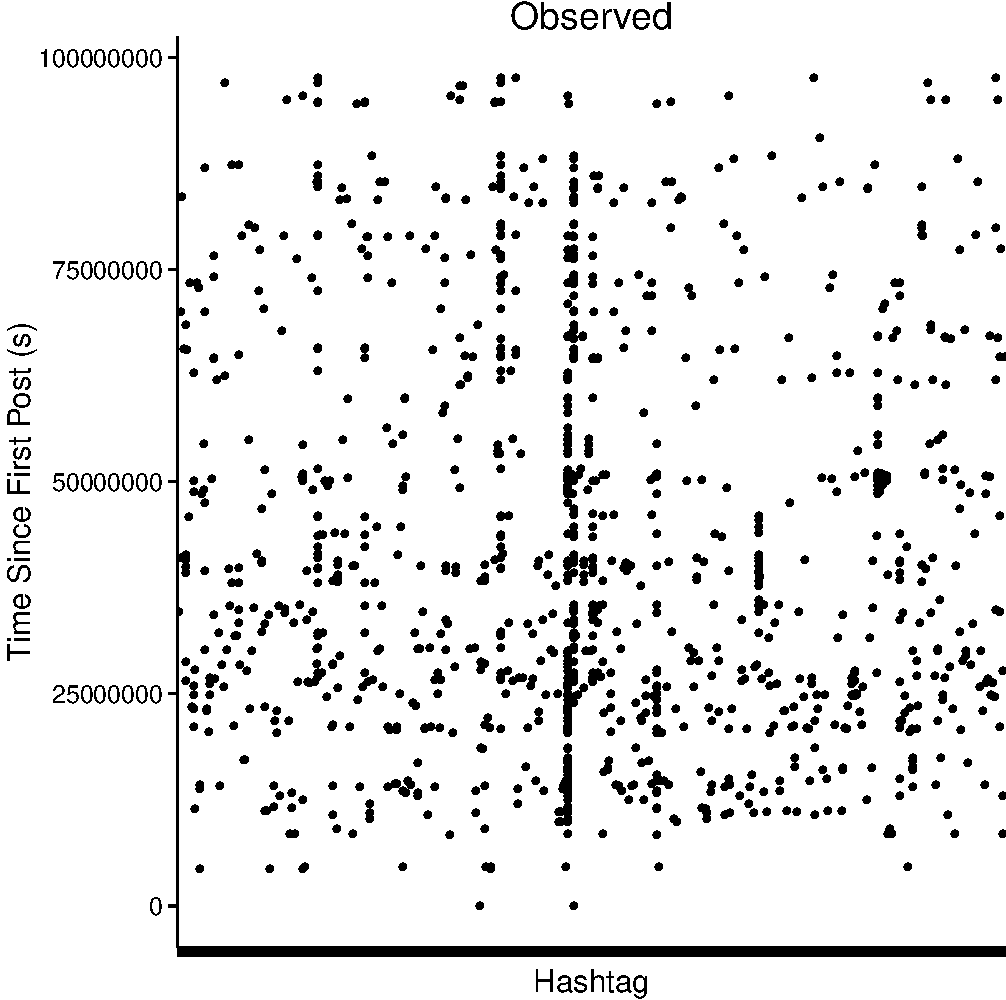
\includegraphics{HTByTime-520957-crop.pdf}}}
  \caption{Tagging profile of a single user on StackOverflow}
  \label{figHTByTime-520957}
\end{figure}

\begin{figure}[!htbp]
  \scalebox{.8}{\resizebox{\linewidth}{!}{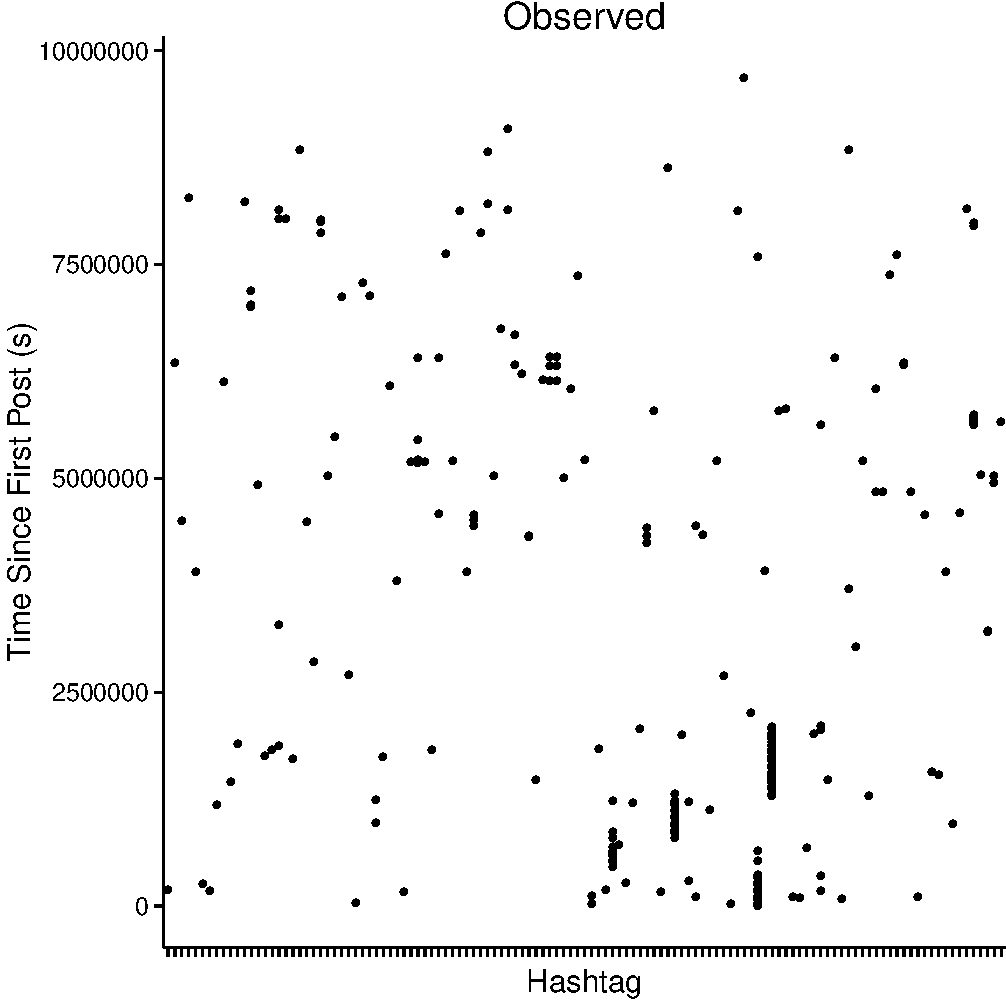
\includegraphics{HTByTime-fashionista_com-crop.pdf}}}
  \caption{Tagging profile of a single user on Twitter}
  \label{figHTByTime-fashionista_com}
\end{figure}

The specific value of the hashtag used for both plots is nominal and not important for this analysis.
What is interesting is how large the tagging space is for these users.
There are bands of commonly-used tags for each user, but there are also instances where new tags are used, and a large percentage of tags used are not in the most-common bands.
This helps illustrate how challenging modeling this task can be.
The model's goal is to predict at each instance what tag will be chosen, but since the tag space is so large and varied, this task is quite challenging.

Although the tag space for the Twitter user is smaller than the StackOverflow user in these plots, this is not a consistent trend.
These plots were chosen from the set to also show that the amount of tag variation for individual users also varies: some use many tags and some use just a few.
To accurately model human performance in this domain, the model must be able to make accurate predictions across all variations of user tagging behavior. 

\subsubsection{Visualizing Model Performance}

As a first method for understanding model performance, profile plots of model's predicted tags for individual users were overlaid on that user's actual tag use.
These plots for StackOverflow and Twitter are included in Figures \ref{figHTMByTime-520957} and \ref{figHTMByTime-fashionista_com} respectively.
These are the same plots shown in Figures \ref{figHTByTime-520957} and \ref{figHTByTime-fashionista_com} with model predictions overlaid in red. 

\begin{figure}[!htbp]
  \scalebox{.8}{\resizebox{\linewidth}{!}{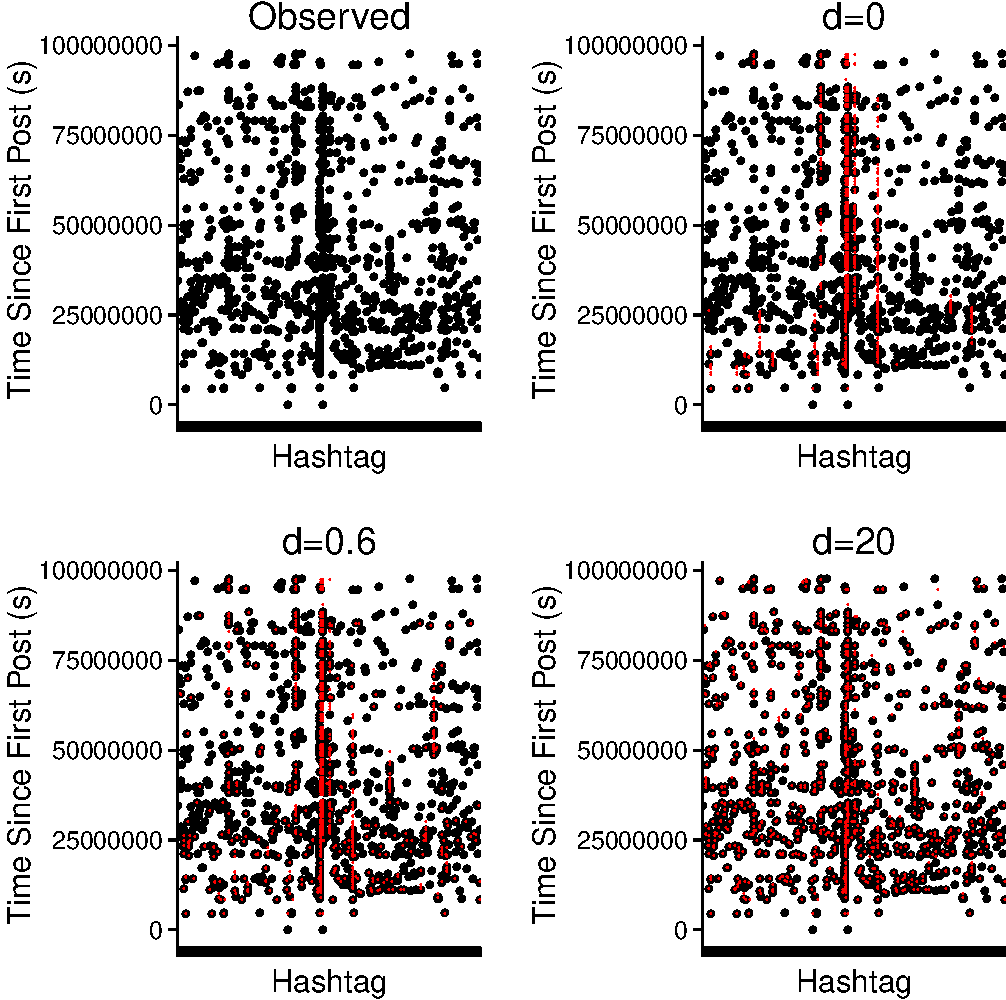
\includegraphics{HTMByTime-520957-crop.pdf}}}
  \caption{Model tagging profile of a single user on StackOverflow}
  \label{figHTMByTime-520957}
\end{figure}

\begin{figure}[!htbp]
  \scalebox{.8}{\resizebox{\linewidth}{!}{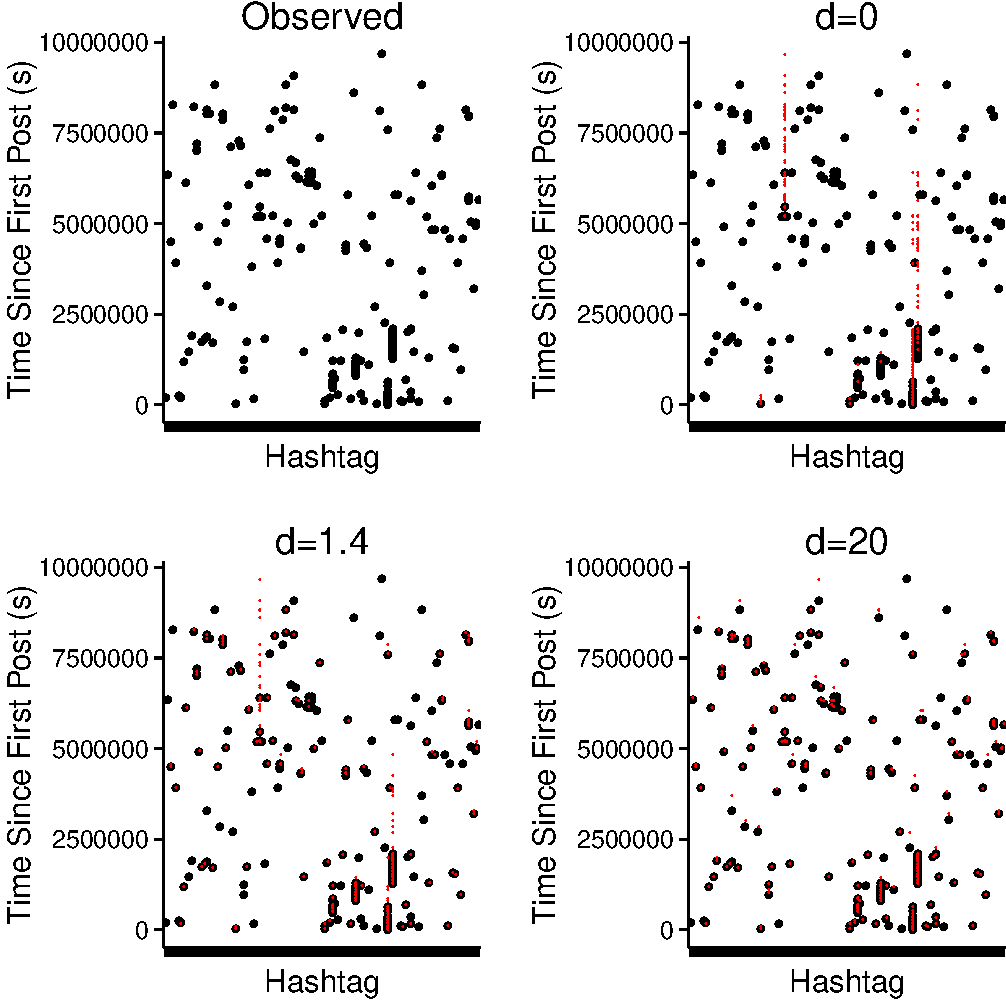
\includegraphics{HTMByTime-fashionista_com-crop.pdf}}}
  \caption{Model tagging profile of a single user on Twitter}
  \label{figHTMByTime-fashionista_com}
\end{figure}

Also shown in these figures is how model predictions change as the decay rate parameter changes.
The model changes less from tag to tag with lower decay rate values.
This makes sense because lower decay rate values lead to the model weighting frequency more than recency in the activation calculation.
These plots also suggest that model accuracy is best when a blend of frequency and recency is used (i.e., a decay rate between 0 and 20).
This will be more formally tested when model accuracy across decay rate values is analyzed across all users in each dataset slice and all dataset slices.

\subsubsection{Model Performance Across Decay Rate Values}

Moving up one level of analysis, model accuracy for all users in a single dataset slice was analyzed.
A plot of the results for one of the 12 slices, for both Twitter and StackOverflow, and for both forms of $B_{i}$ are included in Figures \ref{figPriorSOQSliceDs} and \ref{figPriorTwitterSliceDs} respectively.

\begin{figure}[!htbp]
  \scalebox{.8}{\resizebox{\linewidth}{!}{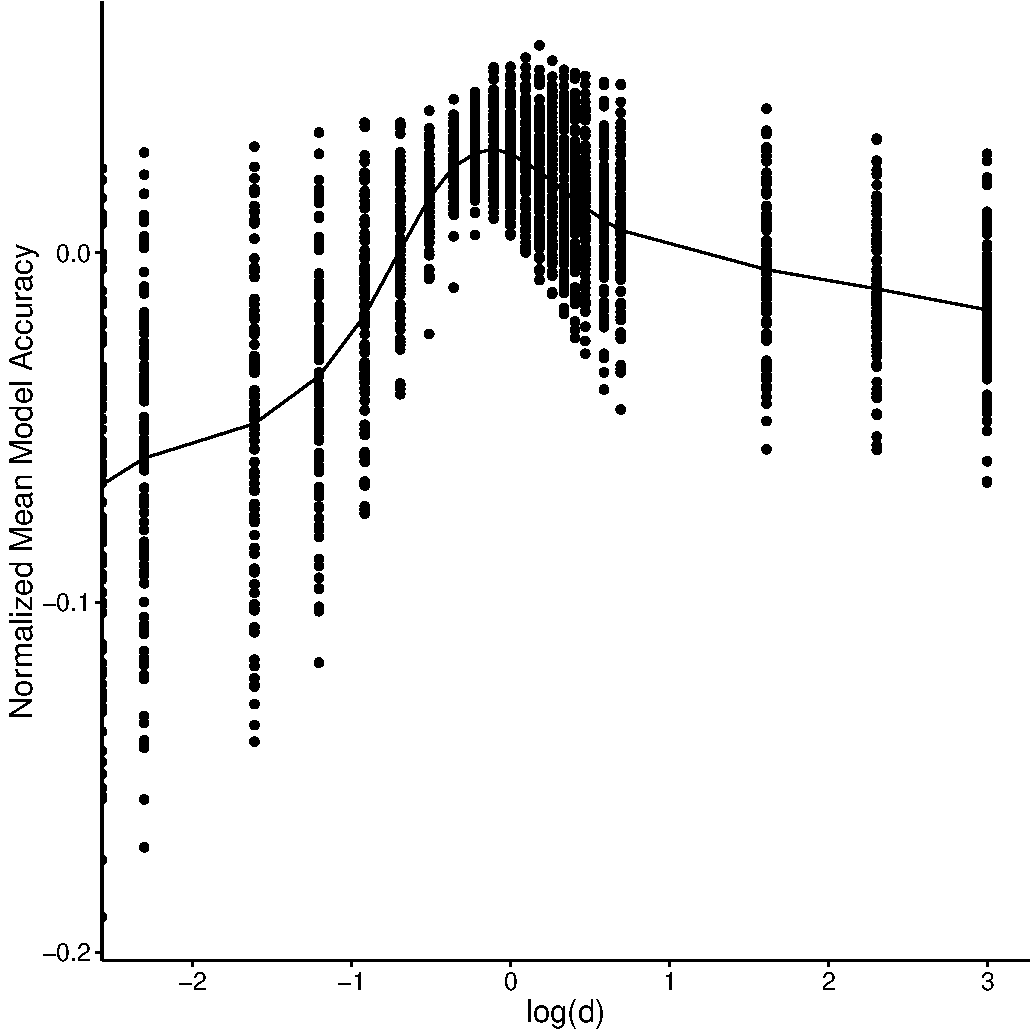
\includegraphics{visNormMean-SOQgt500r2-topHashtagPostPriorStd-crop.pdf}}}
  \caption{Model performance for a single dataset slice for StackOverflow}
  \label{figPriorSOQSliceDsStd}
\end{figure}

\begin{figure}[!htbp]
  \scalebox{.8}{\resizebox{\linewidth}{!}{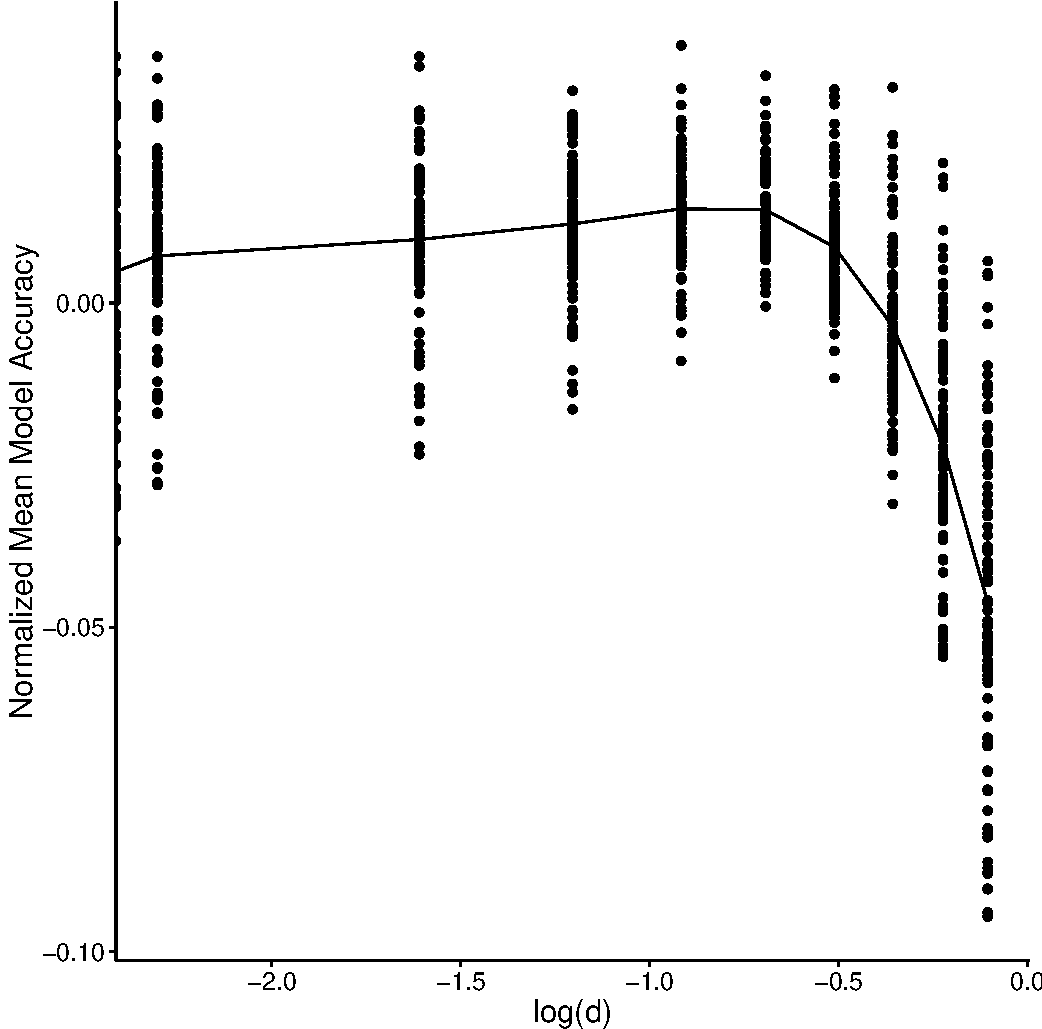
\includegraphics{visNormMean-SOQgt500r2-topHashtagPostPriorOL2-crop.pdf}}}
  \caption{Model performance for a single dataset slice for StackOverflow}
  \label{figPriorSOQSliceDsOL}
\end{figure}

\begin{figure}[!htbp]
  \scalebox{.8}{\resizebox{\linewidth}{!}{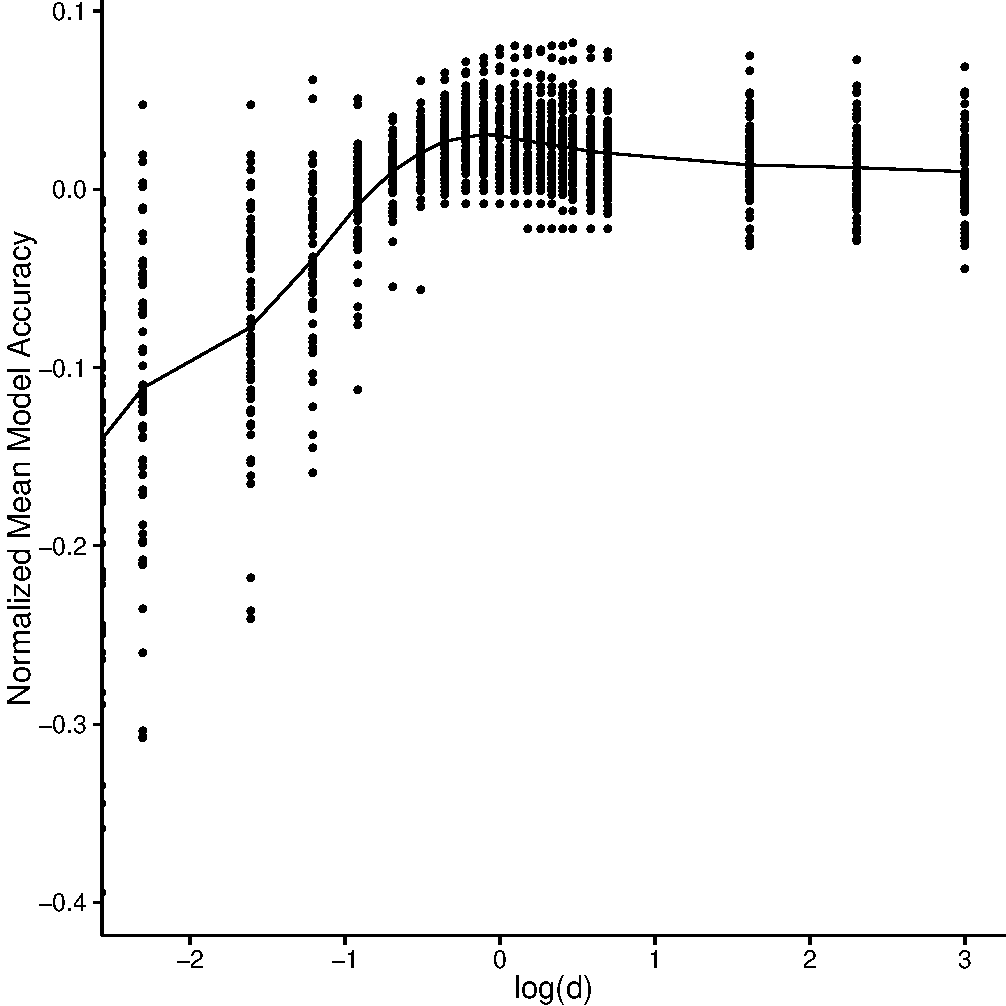
\includegraphics{visNormMean-TFollowgt10Mr2-topHashtagPostPriorStd-crop.pdf}}}
  \caption{Model performance for a single dataset slice for Twitter}
  \label{figPriorTwitterSliceDsStd}
\end{figure}

\begin{figure}[!htbp]
  \scalebox{.8}{\resizebox{\linewidth}{!}{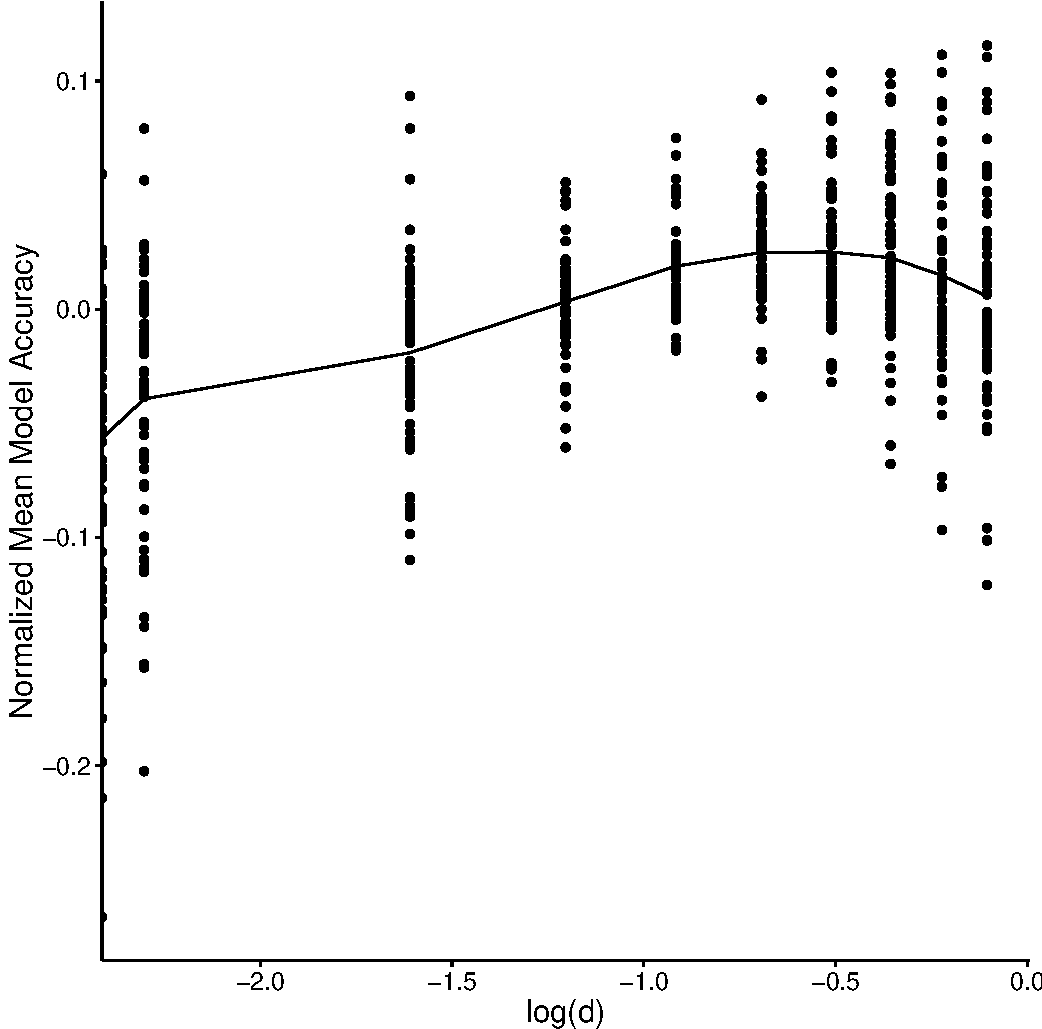
\includegraphics{visNormMean-TFollowgt10Mr2-topHashtagPostPriorOL2-crop.pdf}}}
  \caption{Model performance for a single dataset slice for Twitter}
  \label{figPriorTwitterSliceDsOL}
\end{figure}

Model accuracy at each decay rate value for each user in the dataset slice are included in the plots.
Each user's mean accuracy was subtracted off in order to compute a normalized mean for that user.
This was done so that the relative accuracy change for different decay rate values could be more easily visualized.
The technique is a visualization to what is done when testing the main effect in a repeated measures design.

One main effect in all of the plots is that there is an optimal decay rate value between 0 and 20 that produces the highest model accuracy.
For the standard $B_{i}$ equation, model accuracy for a pure frequency model ($d=0$) is also worse than using a pure recency model ($d=20$), particularly for Twitter.
It makes sense that a pure recency model for Twitter is relatively more accurate than for StackOverflow, as the hashtag lifetime for Twitter is much less than a programming-language tag on StackOverflow.

When comparing the standard and optimized learning forms of the equation, it is apparent that a pure recency model does not work very well for optimized learning.
The best-fit decay rate value for the optimized learning form is also not as clear and pronounced as it is for the standard form (less of a peak).
And the relative accuracy gained from using a pure frequency based model to a blend of frequency and recency is less for the optimized learning form than the standard form of $B_{i}$.

\subsubsection{Best-fit Decay Rate Values}

To identify the best decay rate value for the dataset slices,
each user's best decay rate value was taken and the results are plotted in histogram form in Figures \ref{figPriorSOQHistDs} and \ref{figPriorTwitterSliceDs} respectively.

\begin{figure}[!htbp]
  \scalebox{.8}{\resizebox{\linewidth}{!}{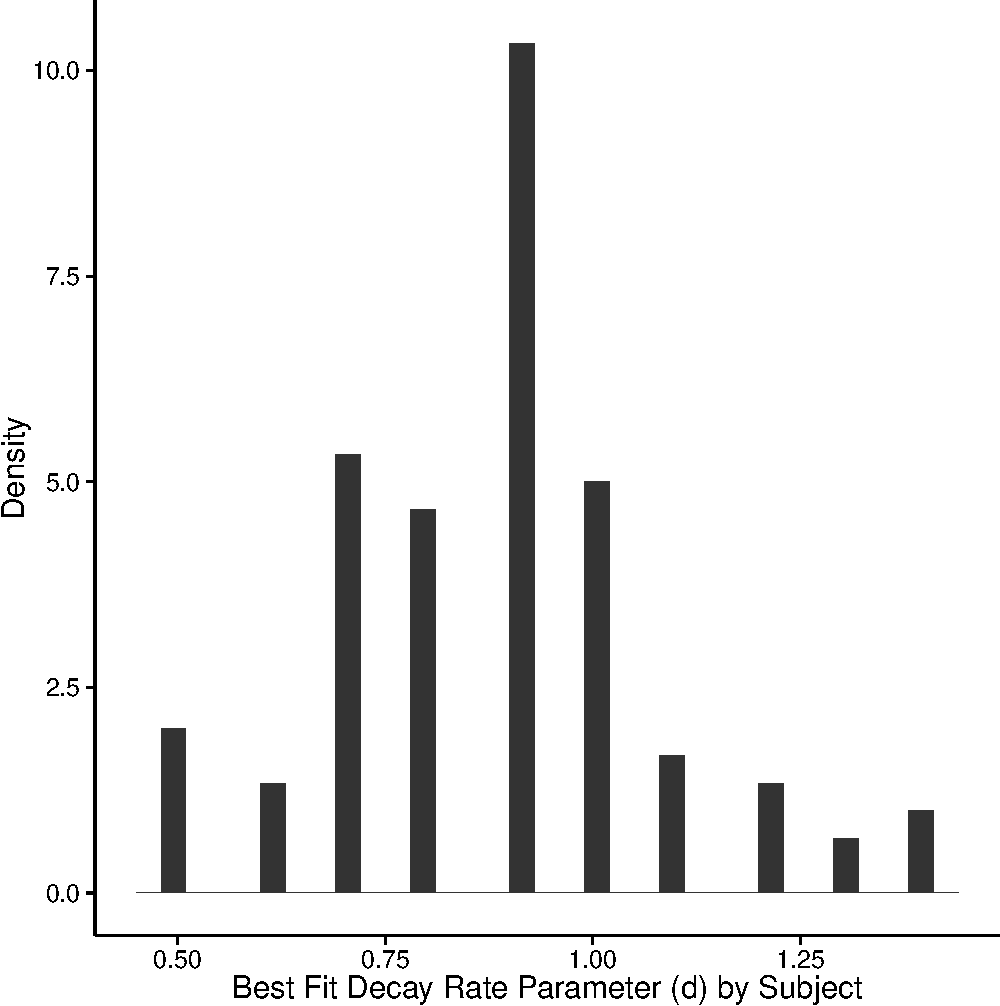
\includegraphics{visHistD-SOQgt500r2-topHashtagPostPriorStd-crop.pdf}}}
  \caption{Best-fit decay rate for a single dataset slice for StackOverflow}
  \label{figPriorSOQHistDs}
\end{figure}

\begin{figure}[!htbp]
  \scalebox{.8}{\resizebox{\linewidth}{!}{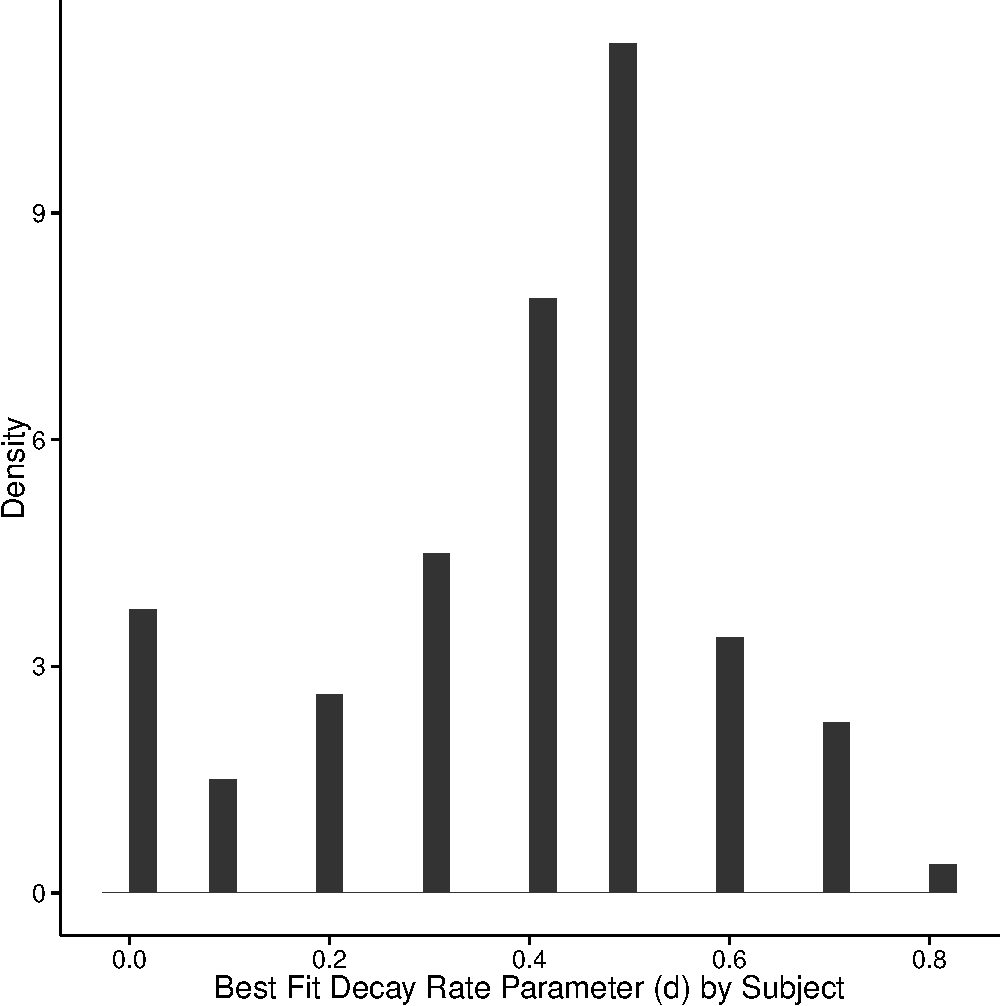
\includegraphics{visHistD-SOQgt500r2-topHashtagPostPriorOL2-crop.pdf}}}
  \caption{Best-fit decay rate for a single dataset slice for StackOverflow}
  \label{figPriorSOQHistDsOL}
\end{figure}

\begin{figure}[!htbp]
  \scalebox{.8}{\resizebox{\linewidth}{!}{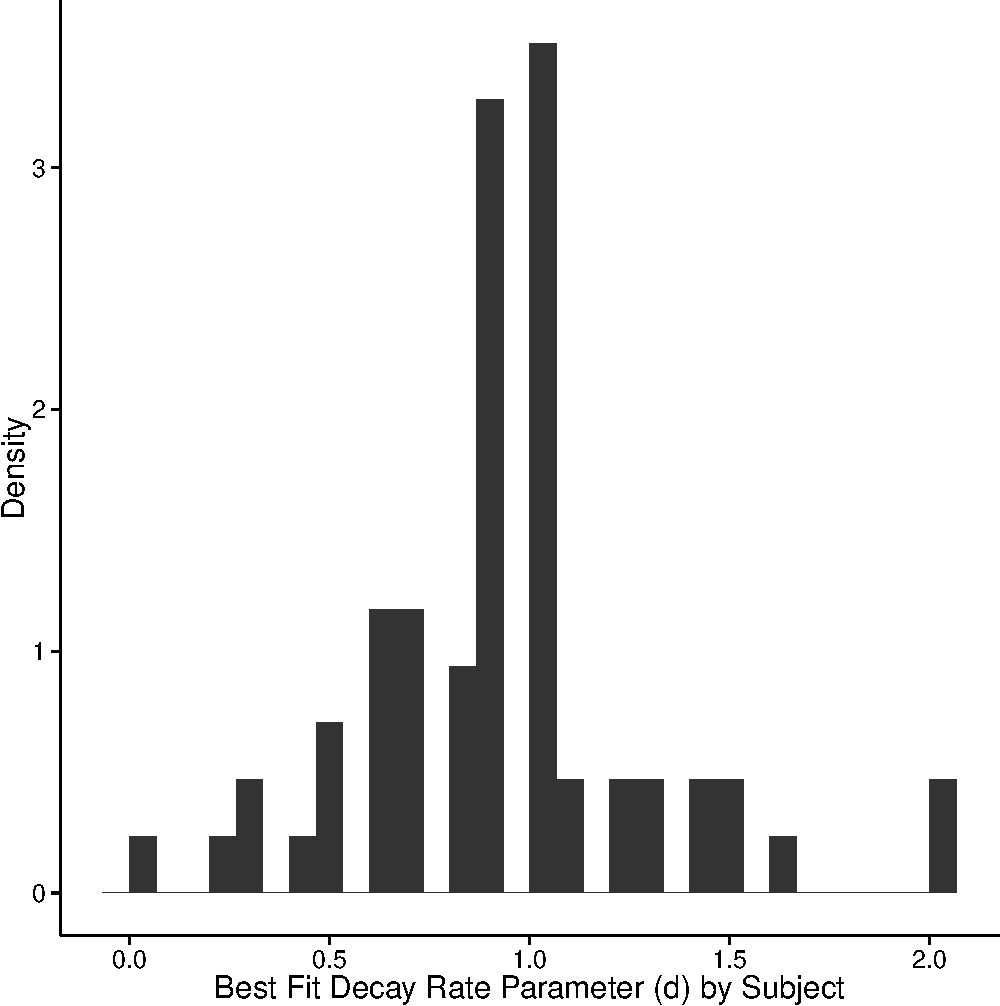
\includegraphics{visHistD-TFollowgt10Mr2-topHashtagPostPriorStd-crop.pdf}}}
  \caption{Best-fit decay rate for a single dataset slice for Twitter}
  \label{figPriorTwitterHistDs}
\end{figure}

\begin{figure}[!htbp]
  \scalebox{.8}{\resizebox{\linewidth}{!}{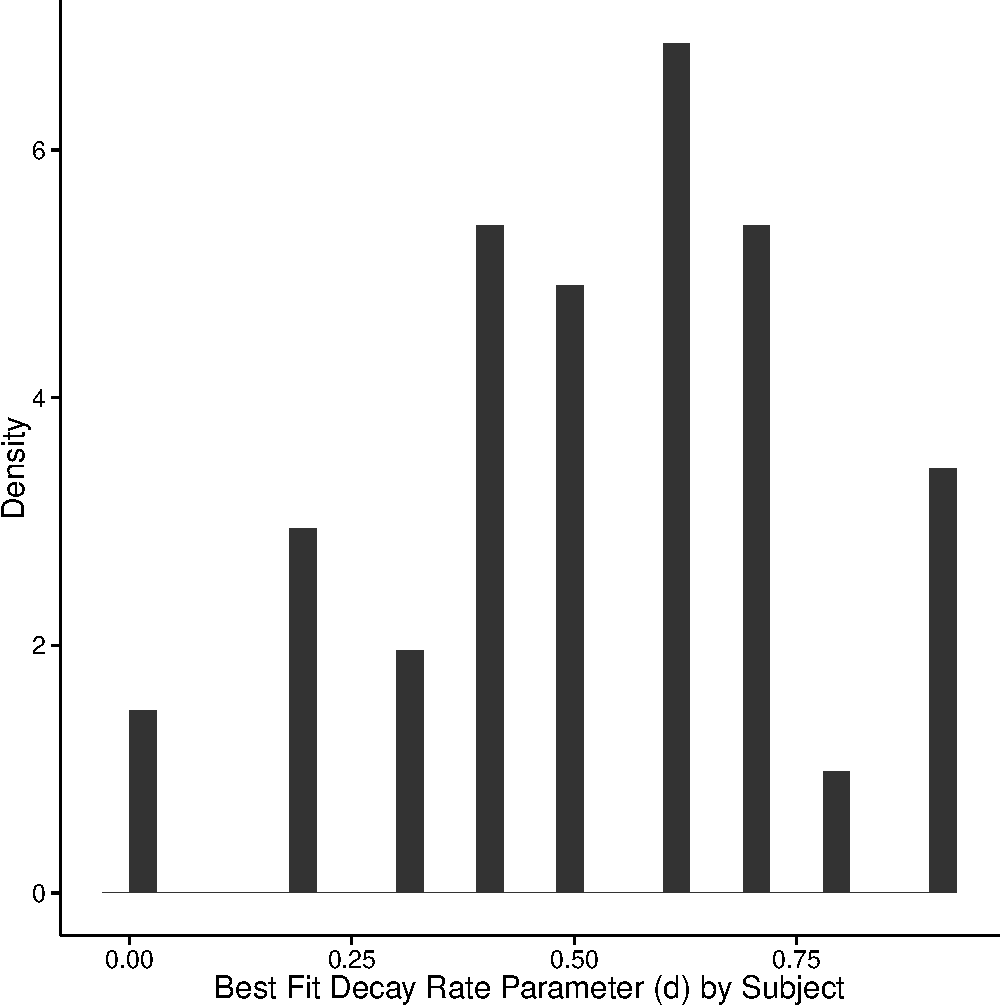
\includegraphics{visHistD-TFollowgt10Mr2-topHashtagPostPriorOL2-crop.pdf}}}
  \caption{Best-fit decay rate for a single dataset slice for Twitter}
  \label{figPriorTwitterHistDsOL}
\end{figure}

First, the best-fit values are close to the 0.5 default value used in ACT-R when the optimized learning form is used.
Comparing across optimized learning and the standard form, the best-fit values for the standard form are slightly higher for both the StackOverflow and Twitter dataset slices.
Comparing best-fit values will be more thoroughly tested when looking at the values across all dataset slices.

\subsubsection{Aggregate Model Performance}

Finally, model accuraccy was analyzed across all dataset slices for StackOverflow and Twitter.
Mean accuracy for both sites is included in Figure \ref{figPriorAcc}. 
The mean was computed by taking the mean of the mean model accuracy for each dataset slice.
All confidence intervals are 95\% bootstrapped for the mean of the means for each slice.

\begin{figure}[!htbp]
  \scalebox{.8}{\resizebox{\linewidth}{!}{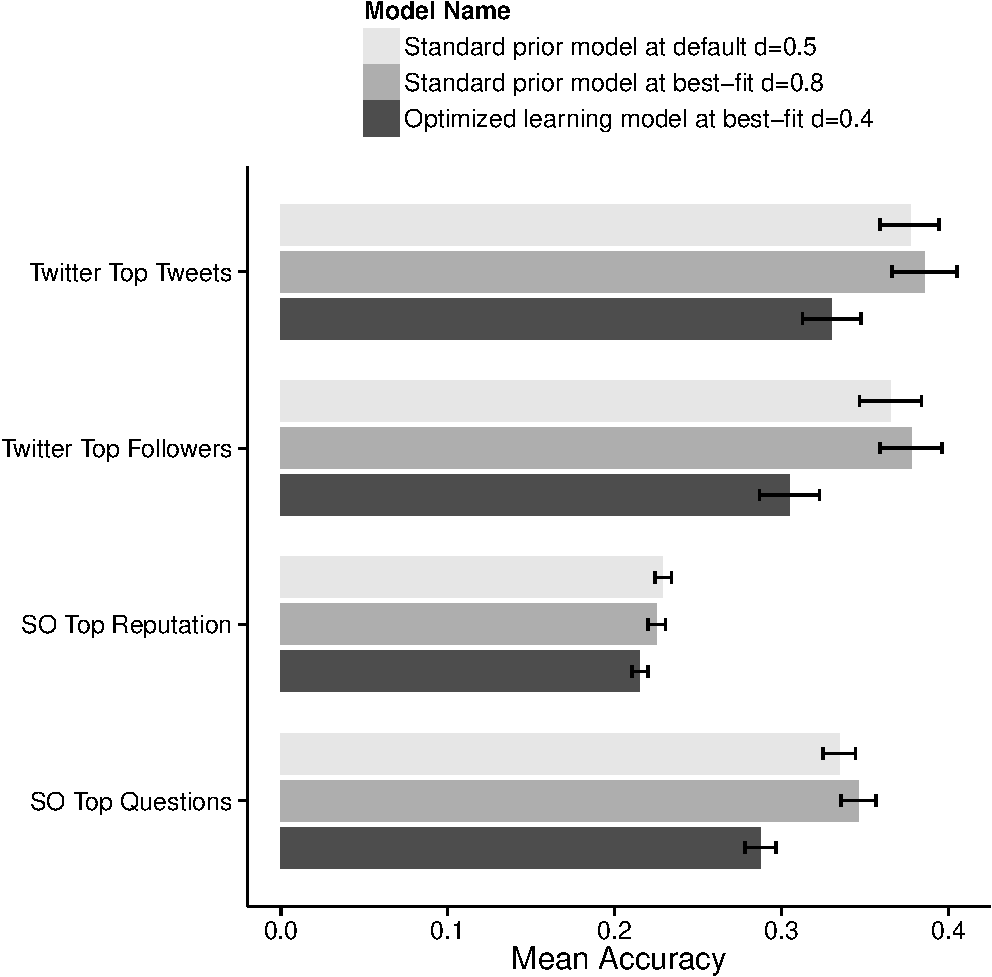
\includegraphics{compareMeanDV-acc--crop.pdf}}}
  \caption{Model accuracy}
  \label{figPriorAcc}
\end{figure}

Accuracy for the standard form (0.35) is higher than the optimized learning form (0.30).
This makes sense given that the standard form does not assume equal presentation rate for each chunk, and hashtags on Twitter in particular show trends of high rate of use and then shift to low rate of use. 
The standard form of $B_{i}$ is able to more accurately account for these trends.

The best-fit decay rate values were also analyzed across all dataset slices.
These results are included in Figure \ref{figPriorDecay}.

\begin{figure}[!htbp]
  \scalebox{.8}{\resizebox{\linewidth}{!}{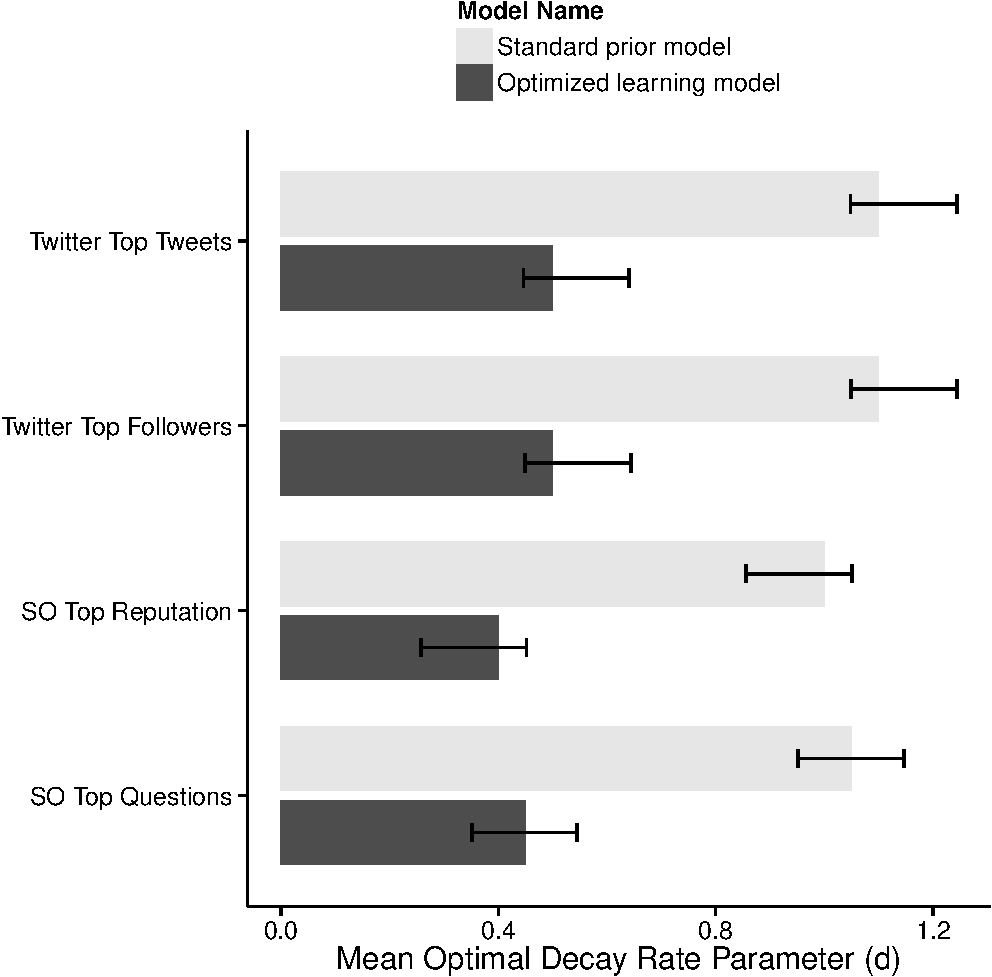
\includegraphics{compareMeanDV-d--crop.pdf}}}
  \caption{Best-fit decay rate}
  \label{figPriorDecay}
\end{figure}

Decay rate values that produced the most accurate model performance are lower for the optimized learning form (0.43) of $B_{i}$ compared to the standard form (0.80).
However, the optimal values for optimized learning are near 0.5, which lines up with default value used in ACT-R.
So the decay rate values for the standard form are slightly higher than the default values used in ACT-R, but the values found when optimized learning is used line up nicely with the ACT-R defaults.

\subsection{Discussion}

Given the large tag space used by post authors on StackOverflow and Twitter, it was surprising that model performance is respectable even when only past tag history and no context is used.
This speaks to the importance of not only taking into account overall past tagging history, but also to ensuring that the prior component of activation for each tag is customized to each user's specific past tagging history.

Also apparent for these datasets is that the optimized learning form of $B_{i}$ is not as accurate as the standard form.
Further, for the optimized learning form there is not much difference between using a pure frequency-based model and a model where frequency and recency are optimally blended.
This makes sense given that the optimized learning equation in Table \ref{tabACTRBLLModel} collapses to a pure frequency model as the amount of time since the presentation of the first recorded chunk instance increases,
and also since the timespan of recorded tag use for StackOverflow and Twitter is large (years).

So it may be worthwhile to use the standard form instead of the optimized learning form when declarative memory is modeled across a broader range of tasks.
However, this shouldn't be taken as a strong recommendation,
since the performance benefits seen here could simply be due to the fact that the declarative memory retrievals span across a large period of time, which isn't the case for all tasks.
Nonetheless, the only real reason not to use the standard form is due to computational resource limitations.
Since this becomes less of an issue as time progresses, it may be worthwhile to reconsider the default value used in ACT-R.
It may be the case that the optimized learning form of the equation is no longer computationally necessary.
And if the standard form is used as the default (or simply tried in another experiment),
the results from this study suggest that the optimal decay rate value should be set slightly higher (0.8) than the default when optimized learning is used (0.5).

\section{Combining Predictors}

The declarative memory models analyzed in this study consist of two main components: past behavior and context.
Past tag use was isolated in the first study to see how well ACT-R's prior component of declarative memory (i.e., base-level learning) fits each user's tag use over time.
However for the rest of the studies the past behavior and context declarative memory components were combined as well as looked at in isolation.

\subsection{Methods}

\subsubsection{Logistic Regression}

In order to best combine these predictors, a logistic regression statistical technique similar to \textcite{Stanley2013} was used to determine the most optimal weights for each term.
Logistic regression is used on these datasets in the following way.
When a user creates a tag for a post, a retrieval request for the model is made.
For each request, the model returns a set of tags (all tags that have been observed for that user in the past) and activations associated with each tag.
An activation value is computed for each model component (e.g., prior tag use, context) for each tag.
These values are recorded, and tag instances that match what the author actually tagged are marked as a 1, while all others are marked with a 0.
This process is repeated across all posts where a user chooses a tag, and across all users in the dataset.
Once all of the results are aggregated, a logistic regression is run where the optimal weights for each model component are found that maximize the model's ability to correctly label tags as 0 or 1 based on total activation.

Model accuracy is evaluated by using the optimal weights, rank ordering all recorded tags by model activation using those weights,
asking the model to tag the top N posts with a 1 (where N is the total number of recorded instances where an author chose a tag),
and then comparing the model's chosen tags with the used tags for each post (i.e., looking at the ``hits'').
This is equivalent to throttling the threshold in the logistic regression such that the total number of observations labeled as a 1 match the total number of recorded instances of tagging in the dataset.

For this form of model accuracy, the model labels N posts with a 1 where the labeling is not constrained in any way within each post.
That is, the labeling is relaxed across all posts, and there are no constraints where the model must label a specific number of 1s for each post based on the number of tags that the author used for that post.
So model accuracy values found with the relaxed method are actually slightly conservative, since the model may be labeling more 1s for a post than the number of tags the author used for that post.

However, this relaxed metric was used for the rest of the experiments that involve combining terms because the optimal weights found by the regression are based on using the relaxed metric.
If these weights are then used to compute the constrained form of model accuracy, biases may be introduced since the regression wasn't optimized to the constrained form, and weights may change if that was done.
The constrained form of model accuracy can not be used for the regression because there is no current logistic regression technique in R that can be constrained to label a specific number of 1s for each observation. 
The constrained form could be used in a regression if a custom form of the regression was implemented.
However this was not persued since around \num{2500} total regressions were run on these datasets for two reasons:
A custom implementation in R would not likely run in compiled C, and even if it was implemented in a compiled language it would be computationally intractible without a closed-form solution. 

\subsubsection{Adding Offset Term}

This logistic regression method is a computationally efficient way to find the optimal weights for the predictors.
However when the regression can not be constrained to label a specific number of 1s for each observation (as is the case here), to be used properly an offset term must be added as an additional model predictor.

The offset term ensures that the activation for the small number of top tags for each post are equal across posts.
This ensures that the logistic regression only labels a few 1s for each post.
\textcite{Stanley2013} did this by subtracting off the mean total activation for the top 5 tags for each post.
However this method is complicated since computing the toal activation for a tag requires already knowing the weights for each model component that are used to compute that activation.
\citeauthor{Stanley2013} used an iterative approach to determine the weights used for the offset term, and kept iterating until those weights matched the weights returned after running the logistic regression.

A simplified version of \citeauthor{Stanley2013}'s method was used for the results in this study.
Instead of subtracting off the mean total activation for the top 5 tags for each post, the process is done in isolation for each model component.
So for the prior component, the activation value used in the logistic regression is the prior activation with the mean of the top 5 prior activations subtracted off of this value.
The same process is used for the context component.
Decoupling the offset term and computing an offset for each model component in isolation means that an iterative approach is no longer necessary,
since the optimal weights of the terms are no longer needed when computing the offset.

\subsubsection{Datasets}

Model accuracy was computed on the popular-hashtags dataset for Twitter and a random sample of posts across the entire StackOverflow dataset.
For each of the four Twitter popular-hashtags datasets, model retrievals were done across 15 runs and 500 posts within each run.
For the StackOverflow dataset, 5 runs of 100 posts were used, since the results for StackOverflow are more stable and retrievals take more wall-clock time for this dataset due to the size of the co-occurrence matrix.
All runs contained separate posts, and all posts used for runs were not used to generate the co-occurrence matrix used for the two retrieval models.

\subsubsection{Computing Prior}

For each randomly-sampled post for StackOverflow, the prior activation is based on that user's prior tagging history, and not on any global prior of specific tag frequency across users.
This was done so that the prior component used for StackOverflow for both the popular-users and randomly-sampled subsets was the same.

However, a custom user prior for the Twitter popular-hashtags dataset cannot be used, since the entire Twitter dataset cannot be downloaded.
This dataset contains samples of a large set of various users that choose a specific set of hashtags being monitored.
So in order to generate a custom user prior for each sample in the dataset, that user's entire tagging history must be accessed through the API.
Since access rates are limited across that interface, it is infeasable to do this process for every user that appears in the Twitter popular-users dataset.
So instead, the global prior tag history for all users in the Twitter popular-users dataset was used to compute prior activation values for each tag.

\subsubsection{Co-occurrence Matrices}

The context component for both the Random Permutation and Bayesian model requires a co-occurrence matrix of words and observed tags.
Different size matrices were analyzed, ranging from \num{1000}, \num{10000}, \num{100000}, \num{1000000}, and \num{3000000} posts.
The matrix for \num{3000000} posts was only used for Twitter, since the number of words in a StackOverflow post is much higher than Twitter on average,
and the space and computational time required when using a co-occurrence matrix of \num{3000000} posts for StackOverflow is too high for a current high-performance desktop, even with highly optimized representations.
Already FIXME total co-occuring word tag observations are used to build a co-occurrence matrix of \num{1000000} StackOverflow posts.
It is also the case that \num{1000000} posts for StackOverflow is already around $1/7$ of the total posts created on the site,
so it is reasonable to assume that the results would not change greatly for StackOverflow if $3/7$ of the total posts created were used to build the co-occurrent matrix instead,
especially since FIXME co-occurrences are already used with \num{1000000} posts.

\section{Results for Combining Terms}



\subsection{Adding Offset}

Model accuracy relaxed across posts with and without the offset model component was evaluated for both the Bayesian and random-permutation model.

\subsubsection{Method}

The four Twitter popular-users datasets and the StackOverflow randomly-sampled dataset were used for the analysis.
Logistic regressions were run both with and without the offset component added to each model.
The results for each run for each dataset were collected and averaged.
The results across the four Twitter datasets were collected together, and the average was done across all runs in all four datasets.

\subsubsection{Results}

The impact of adding the offset to each of the models for StackOverflow and Twitter are included in Figures \ref{figContextOffsetSO} and \ref{figContextOffsetTwitter}.


\begin{figure}[!htbp]
  \scalebox{.8}{\resizebox{\linewidth}{!}{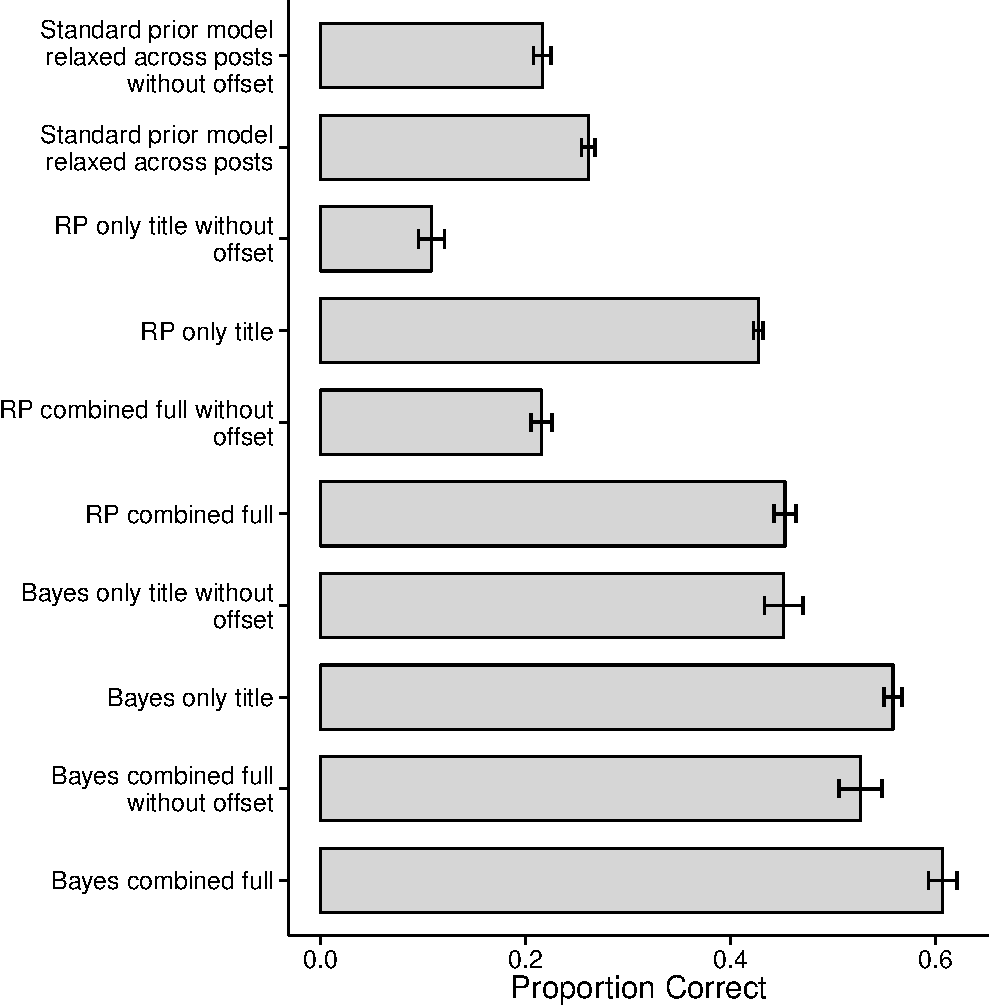
\includegraphics{compareMeanDV-acc-OffsetSO-crop.pdf}}}
  \caption{Impact of adding model offset for StackOverflow}
  \label{figContextOffsetSO}
\end{figure}

\begin{figure}[!htbp]
  \scalebox{.8}{\resizebox{\linewidth}{!}{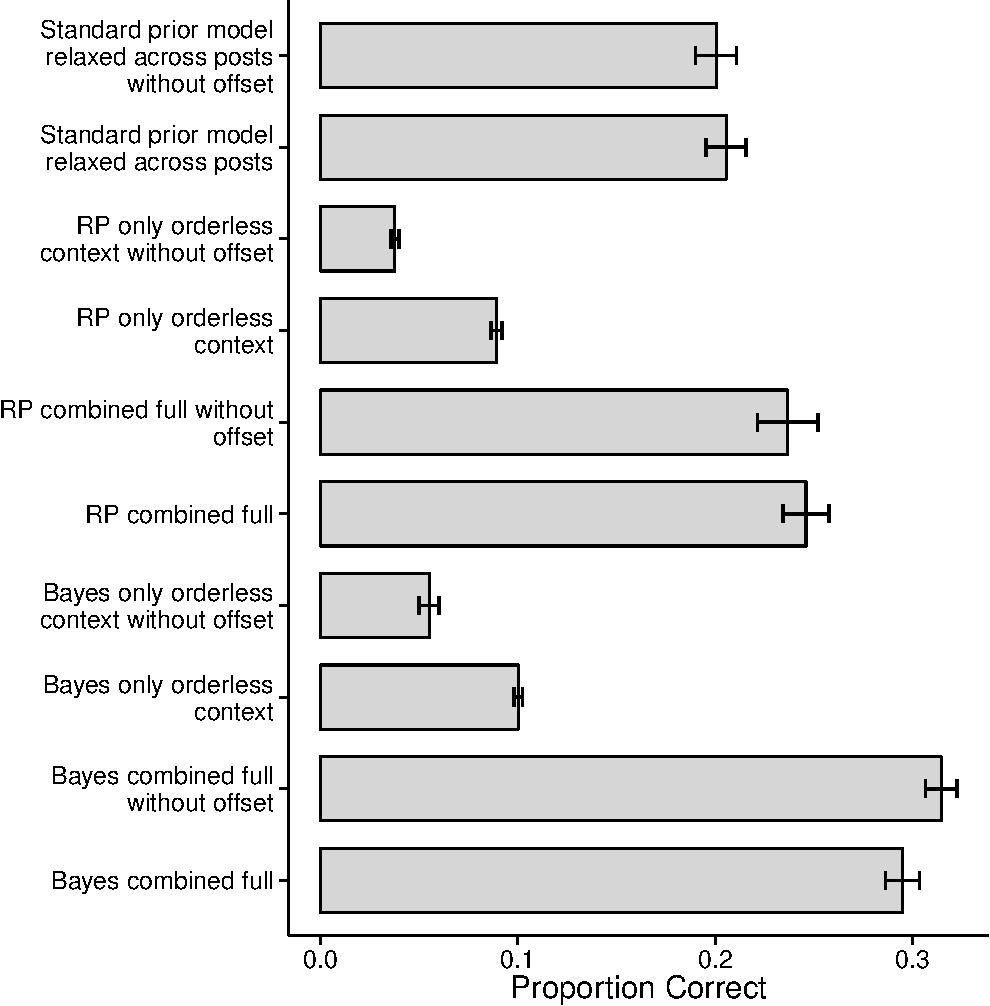
\includegraphics{compareMeanDV-acc-OffsetT-crop.pdf}}}
  \caption{Impact of adding model offset for Twitter}
  \label{figContextOffsetT}
\end{figure}

In both plots, if the model name includes ``full'' then all model components are included.
When they are enumerated, then components are left out.
The random-permutation models are represented as ``RP'', Bayesian models as ``Bayes'', and they are plotted alongside each other so that comparisons across the two model types can be done easily.
So, for example, the ``standard Prior model relaxed across posts w/o offset'' means that only the prior model component was used, and the offset for that component was not subtracted off when determining activation.
As another example, the ``Bayes only orderless context'' means that only the context component of the Bayesian model was used (along with the offset), and that no order information was used for that contextual component term.

Looking across the plots, including the offset significantly increases model accuracy, for all models, terms, and sites.
Accuracy is improved even when only a single term is used.
Although in this case the weight of the term is irrelevant (only one term, weighting for that term doesn't matter),
using an offset still improves accuracy since the offset term ensures that only a small number of tags per posts are predicted by the model to be the chosen tags. 

The random-permutation model in particular is greatly affected by the offset term, for both the StackOverflow and Twitter.
This suggests that the mean activation for the random-permutation model for the top few tags in each post can vary greatly across posts.
Only if this mean activation is subtracted off will the logistic regression model generate optimal weights and predictions that are comparative to the Bayesian model when model accuracy relaxed across posts is examined.

\subsubsection{Discussion}

It is actually somewhat dissapointing that the offset term is even needed.
If it were the case that model activation for a tag in a specific post could be interpreted as an exact activation value that did not depend on the specific post,
then the model would be able to say when, for example, the third top tag in a post is more likely to be a chosen tag than the second top tag in another post.
That is, the activation values would have meaning more than just rank ordering, and could be used to determine, for example, the number of retrievals to do for a specific post.
If this were the case, then adding the offset term would actually decrease accuracy, since this absolute value of the activation values would be subtracted off.
However, since accuracy improves when adding the offset term for both models, it does not seem that activation values have much meaning across posts (and only within a single post) for these datasets.

A likely and simple explaination for this is that possibly there are posts where a large set of tags have high activation,
but the author is throttling their retrieval threshold for each post such that only a small set of tags are actually used.
This is probably not the retrieval threshold used in the core declarative memory system that determines if a retrieval for the term actually happens.
It is unlikely that this retrieval threshold can be directly controlled and manipulated.
Rather, it could be a high-level task retrieval threshold that the author has control over, where he/she actively sets it based on competing goals of tagging posts an not overly saturating a post with tags.
Adding the offset term into the model is a way to implement a simple version of this high-level retrieval threshold.

\subsection{Twitter Subsets}

Four subsets of the popular-users dataset were collected for Twitter.
This was to ensure that model results could be interpreted as effects that were not specific to a certain time period or set of popular hashtags.

\subsubsection{Method}

The four subsets were collected across a period of one month.
The hashtags used in each subset were chosen by scraping a site that published the current trending hashtags for each city.
Hashtags for each US city were collected, and then 400 were randomly sampled from this set.
Only 400 were selected since this is the maximum that the Twitter API can monitor at one time.

\subsubsection{Results}

A plot of model accuracy for components of both the Random Permutation and Bayesian models and isolated by Twitter popular-users subset are included in Figure \ref{figContextSubsets}.

\begin{figure}[!htbp]
  \scalebox{.8}{\resizebox{\linewidth}{!}{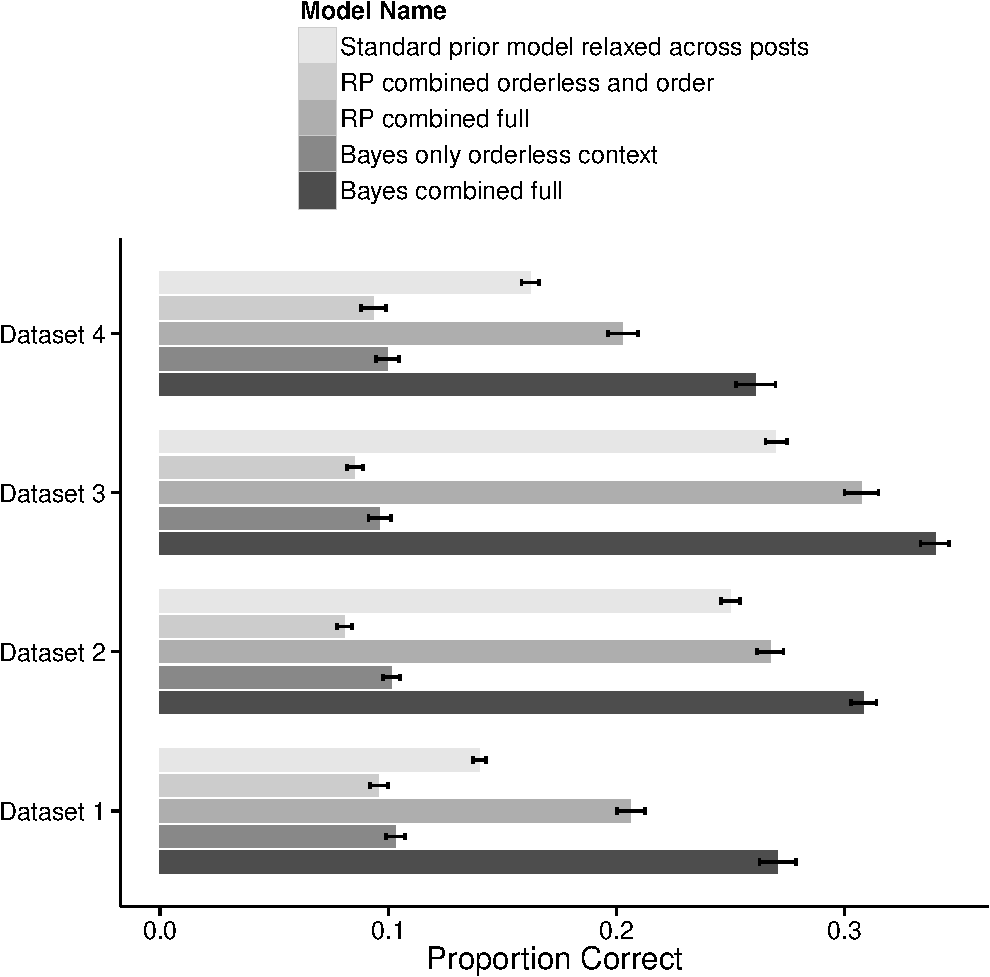
\includegraphics{compareMeanDV-acc-contextStandardByGroupT-crop.pdf}}}
  \caption{Model accuracy for each of the four Twitter popular-users subsets}
  \label{figContextSubsets}
\end{figure}

Although there is a main effect of subset, there are minimal to no practically significant interactions.
Relative model performance remains consistent across the four subsets.

\subsubsection{Discussion}

Since the interactions across popular-users datasets are minimal, model behavior for the popular-users subset for Twitter can be interpreted as behavior that will persist across different time periods,
if the same method of choosing popular hashtags is done at a later date.
It may be more general that model behavior also does not depend on the specific method of choosing the popular hashtags, but since only a single method was used for this analysis,
the results from this study cannot by themselves be used to answer this question.

\subsection{Stop Words}

\textcite{Sahlgren2008} looked at several ways to handle the commonly-occurring stop words for the random-permutation model:
A data-driven frequency-weighted approach was tried, along with using a previously-derived stoplist, and no stop word removal at all.
Removing the high-frequency words in the dataset showed the highest performance increase compared to no stop word removal, and uing a previously-derived stoplist hardly increased performance.
However, \citeauthor{Sahlgren2008} did not try to weight the stop words, and only tried methods to remove them.
So alongside looking at frequency weighting, previously derived, and no stop word removal, \textcite{Stanley2013}'s method of attentuating stop words based on Entropy was also explored.

\subsubsection{Method}

The runs from the Twitter popular-users and StackOverflow randomly-sampled datasets were used for the analysis.
Both the random permutation and Bayesian models were tested.
Activations for context were computed by using the two methods for stop word removal, the entropy weighting method, and no method (i.e., no stop word processing).

\paragraph{Determing Frequency Cutoff}

The same previously-derived stoplist from FIXME that \textcite{Sahlgren2008} used was used for this analysis,
The same entropy weighting method using by \textcite{Stanley2013} was examined,
and the same method of removing the high-frequency words from \citeauthor{Sahlgren2008} was used.

However a cutoff point must be identified and used in order to remove the high-frequency words.
\textcite{Sahlgren2008} used a cutoff where words that occurred more than \num{15000} times were removed.
Since the StackOverflow and Twitter datasets are much larger than the datasets used by \citeauthor{Sahlgren2008}, the same cutoff could not be used.
The ideal cutoff was determined by choosing the value where the standard deviation of the counts for each word for each of the tags were all relatively small.
That is, the spikes were suppressed for standard deviations for particular tags that still contained words with a very large number of observations.
The cutoff was also chosen such that the size of the spikes was about as large as the spikes generated when the entropy method was used.

The plot of the standard deviations across tags that was used to identify the cutoff for StackOverflow and Twitter is included in Figures \ref{figContextCutoffSO} and \ref{figContextCuttoffT}.

FIXME:

The no-removal plot shows the size of the spikes when high-frequency words are removed.
The entropy plot shows how the size decreases by more than an order of magnitude when the entropy weighting measure is used.
The cutoff was chosen such that the frequency plot looks similar to the entropy plot, with spikes around the same size.
Note that using a previously-defined stoplist does not remove some of the remaining high-frequency words in these datasets, which hints that this method may not be ideal when model accuracy is examined.
The cuttoff that produced the frequency plot is where a word represents more than \num{.0004} occurrences in the dataset.
This may or may not be equal to the value for \textcite{Sahlgren2008}, since that number was expressed in total observations (not as a percentage), and the total number of words in the dataset were not given.

Also, no strong claims are being made that the cutoff identified is the ideal frequency percentage cutoff for all datasets when a frequency cutoff is used.
The method used to identify this cutoff was simply aimed to find a reasonable value where comparisons between a frequency cutoff and entropy weighting techniques would be equitable.







\subsubsection{Results}

\subsection{Dataset Size}

\subsubsection{Method}
\subsubsection{Results}

\subsection{Amount of Compression for Random Permutation}

\subsubsection{Method}
\subsubsection{Results}

\subsection{Method to Combine Prior and Context}

How can prior likelihood of a user choosing a particular tag be incorporated in the random permutations vector-based model?
Currently vector-based models generate activations for each tag that are based purely on context.
That is, if a particular tag has been used 10 times more often than the other tags by a specific user, that information is not included in a vector-based model.
It seems plausible that performance should improve for vector-based models if this prior tag activation is included.
Adding a prior activation term for the Bayesian StackOverflow model certainly improved performance \parencite{Stanley2013}.
So a method to incorporate a user's prior tag history into a random permutation model will be developed and then tested on the full StackOverflow dataset and Twitter popular-users dataset.

One straightforward way to include a user's prior tag history into a random permutation model is to include ACT-R's base-level activation term ($B_{i}$) as an additional term in the model.
However, this may not be the most mathematically appropriate thing to do, since base-level activation is represented as a log odds value,
and the single strength of association term in a random permutation model is computed by a correlation.
It may be more appropriate to somehow attenuate the memory vectors over time,
so that an association between a word in a post and a tag (i.e., a memory vector) that has long passed is no longer included in that memory vector's representation.
I will try these ideas and any others that are discovered during the model development process, and the one that is the most cognitively plausible and accurate will be chosen.

\subsubsection{Method}
\subsubsection{Results}

\subsection{Word Order}

\subsubsection{Method}
\subsubsection{Results}

\subsection{Impact of Prior vs Context}

\subsubsection{Method}
\subsubsection{Results}

\subsection{User-customized Co-occurrence Matrix}

\subsubsection{Method}
\subsubsection{Results}

\section{General Discussion}

\section{Summary}

This research has numerous components that are relevant to improving our understanding of declarative memory.
It should be emphasized that it has only recently become possible to evaluate psychological theories of declarative memory on large-scale real-world tasks where the theory can be tested on hundreds of millions of data points.
These information-rich large-scale environments provide a unique opportunity to really stress test and explore the impacts of the psychological constraints of each theory
on a much larger scale than has previously been possible.
This environment will allow, for example, overall performance differences between an ACT-R Bayesian retrieval model and a random-permutation vector-based model to be directly compared on two real-world tagging tasks,
which has not been done previously.

This data-rich environment will also enable the proposed modifications to each model to be quickly evaluated, so that further model improvements can be iteratively proposed and tested.
The main two proposed model modifications (incorporating word order into ACT-R and user history into vector-based representations) have not been tested before, and seem likely to significantly improve performance.

Further, the proposed model modifications are aimed at the architectural level, may very well be task independent, and may generalize and improve model fit across other tasks.
Discovering an effective way to represent the time decay of information in a vector-based model could improve model fit on other tasks where the memory model has been used. 
Finding a task-agnostic way to represent word order information in a Bayesian ACT-R model could improve model accuracy when applied to other domains where it seems plausible that participants are utilizing word order.

Additionally, the tag-recommendation models developed through this research should be immediately relevant to real-world tasks.
If model accuracy is high enough, then the developed models may be used as a foundation for tag recommendation systems that are deployed on Twitter or StackOverflow.

Also since the developed models will be task agnostic, they can potentially be used as tag recommendation systems for other domains.
Examples of similar tagging tasks are hashtag use on Facebook, flagging (i.e., tagging) Wikipedia articles for content issues or overly-opinionated material,
auto labeling incoming mail and placing it into appropriate folders, and spam filtering.
Having an accurate and efficient co-occurrence memory model that correctly retrieves relevant tags can be applied to a wide variety of real-world tasks.

The end result of this research will be [1] a better understanding of how a user's past tagging history influences future tag use,
[2] a more thorough evaluation of the strengths, weaknesses, and differences between two cognitively-plausible memory models on large-scale real-world retrieval tasks,
[3] improvements to each memory model where the strengths of each model (word order and user prior likelihood) are incorporated into the other,
and [4] two efficient implementations of the models for making user-customized tag predictions for StackOverflow posts and Twitter tweets. 
Introducing, exploring, and evaluating reasonable architectural modifications to two commonly-used memory models is worth the effort:
It will increase our understanding of how the effects of imposing specific architectural constraints on memory models influence what information is retrieved.

\begingroup
\setstretch{1}
\setlength\bibitemsep{12pt}
\clearpage
\printbibliography[heading=bibintoc]
\endgroup

\end{document}

